\documentclass[10pt,sigconf,anonymous,nonacm]{acmart}

% acmart defines balance as an internal xkeyval key rather than a class
% option.  Set it through the class key interface so the final two columns
% are left unbalanced without producing an unused-option warning.
\makeatletter
\setkeys{acmart.cls}{balance=false}
\makeatother

\settopmatter{printfolios=true,printacmref=false}
\usepackage{amsmath}
\usepackage{algpseudocode}
\usepackage{array,graphicx,textcomp,xcolor,xurl}
\usepackage{amsthm}
\usepackage{dsfont}
\usepackage{booktabs,tabularx,multirow}
\usepackage{tikz}
\usetikzlibrary{arrows.meta,calc,positioning}

\newif\ifshowcomments
\showcommentsfalse
\newcommand{\zmm}[1]{\ifshowcomments{\color{purple}{\{zmm: #1\}}}\fi}
\newcommand{\zmmmod}[1]{{\color{black}{#1}}}
\newcommand{\revise}[1]{{\color{black}{#1}}}
\newcommand{\todo}[1]{{\color{red}{\{Todo: #1\}}}}
\newcommand{\ignore}[1]{}
\newcommand{\etal}{et al. }
\newcommand{\ie}{i.e., }
\newcommand{\eg}{e.g., }

\hypersetup{pdfauthor={}}

% acmart's sigconf format uses flush-bottom columns; retain that behavior so
% short columns do not leave visible gaps at the foot of a page.
\flushbottom
\hbadness=10000
\vbadness=10000

% Keep the ACM two-column float layout compact.  The manuscript contains
% several short tables and algorithm listings; the class default separation
% leaves visibly large gaps below top-of-column floats.  These lengths affect
% only float-to-text spacing, not the template's margins, columns, or type.
\AtBeginDocument{%
  \setlength{\textfloatsep}{8pt plus 2pt minus 2pt}%
  \setlength{\dbltextfloatsep}{8pt plus 2pt minus 2pt}%
  \setlength{\floatsep}{6pt plus 2pt minus 2pt}%
  \setlength{\dblfloatsep}{6pt plus 2pt minus 2pt}%
  \setlength{\intextsep}{6pt plus 2pt minus 2pt}%
}

\newtheorem{theorem}{Theorem}
\newtheorem{proposition}{Proposition}
\newtheorem{definition}{Definition}

\newcommand{\ind}{\mathds{1}}
\newcommand{\code}{\mathrm{Code}}
\newcommand{\ir}{\mathrm{IR}}
\newcommand{\normrule}{\mathrm{NormRule}}
\newcommand{\Rkw}{\mathcal{R}_{\mathrm{kw}}}
\newcommand{\smech}{\sigma_{\mathrm{mech}}}
\newcommand{\Tv}{\mathcal{T}_{\mathcal{V}}}
\newcommand{\Lrec}{\mathcal{L}_{\mathrm{recall}}}
\newcommand{\Lcode}{\mathcal{L}_{\mathrm{code}}}
\newcommand{\Ltot}{\mathcal{L}_{\mathrm{total}}}
\newcommand{\Nviol}{N_{\mathrm{viol}}}
\newcommand{\NTpend}{\bot_{\mathrm{NT}}^{\mathrm{pend}}}
\newcommand{\NTlog}{\bot_{\mathrm{NT}}^{\mathrm{log}}}
\newcommand{\RL}{\mathcal{R}_L}
\newcommand{\RLcov}{\mathcal{R}_L^{\mathrm{cov}}}
\newcommand{\RLunc}{\mathcal{R}_L^{\mathrm{uncov}}}
\newcommand{\RN}{\mathcal{R}_N}
\newcommand{\RU}{\mathcal{R}_U}

\newcolumntype{L}[1]{>{\raggedright\arraybackslash}p{#1}}
\newcolumntype{C}[1]{>{\centering\arraybackslash}p{#1}}
\newcolumntype{R}[1]{>{\raggedleft\arraybackslash}p{#1}}

\newcommand{\paperfig}[2]{%
  \IfFileExists{#1}{%
    \includegraphics[width=\linewidth]{#1}%
  }{%
    \fbox{\parbox[c][3.2cm][c]{0.94\linewidth}{\centering
      \textit{[figure placeholder --- add:}\\[0.2em]
      {\ttfamily\footnotesize \detokenize{#1}}\textit{]}\\[0.5em]
      \footnotesize #2}}%
  }%
}

\title{From Web PKI Norms to Compliance-Checking Code: End-to-End Generation of Auditable Linters}

\begin{document}
\begin{abstract}
Web PKI trust depends on correctly issued certificates. Certificate
linters such as zlint enforce this trust, but PKI experts must still implement
and maintain certificate lints as Web PKI normative sources evolve. This manual process
is increasingly difficult to scale as pre-issuance linting becomes mandatory and
certificate lifetimes shorten. The ecosystem lacks a systematic way to translate
natural-language normative text into lint code, including a principled method to
determine which normative rules are observable from one certificate alone. We present an
end-to-end framework that extracts normative rules from Web PKI normative sources,
determines their lintability, and generates auditable lint code. A dual-layer
extraction pipeline combines deterministic normative-rule recall with
schema-constrained LLM parsing into an intermediate
representation. A four-condition criterion then determines lintability from
the intermediate representation. Restricted code
generation maps supported normative rules to a closed, typed DSL tree converts to Go lint code. On RFC~5280 and the CA/Browser Forum Baseline Requirements, the framework
recalls 2,080 candidate records for normative rules and retains 1,567 as normative rules through its
adjudication procedure. Of these,
278 (17.7\%) are lintable as certificate lints. The manually verified generated lints identify 10 manually confirmed
finding classes across 2,766 certificates in a scan of one million Bugzilla
certificate files.

\end{abstract}

\begin{CCSXML}
<ccs2012>
   <concept>
      <concept_id>10002978.10003014</concept_id>
      <concept_desc>Security and privacy~Network security</concept_desc>
      <concept_significance>500</concept_significance>
   </concept>
   <concept>
      <concept_id>10011007.10011006.10011041.10011047</concept_id>
      <concept_desc>Software and its engineering~Source code generation</concept_desc>
      <concept_significance>300</concept_significance>
   </concept>
   <concept>
      <concept_id>10011007.10011074.10011099</concept_id>
      <concept_desc>Software and its engineering~Software verification and validation</concept_desc>
      <concept_significance>100</concept_significance>
   </concept>
</ccs2012>
\end{CCSXML}
\ccsdesc[500]{Security and privacy~Network security}
\ccsdesc[300]{Software and its engineering~Source code generation}
\ccsdesc[100]{Software and its engineering~Software verification and validation}
\keywords{Web PKI, X.509 certificates, constrained extraction, lintability analysis}
\maketitle

%-------------------------------------------------------------------------------
\section{Introduction}
\label{sec:intro}
%-------------------------------------------------------------------------------

The Public Key Infrastructure (PKI) forms the trust foundation of the Internet, enabling identity authentication and encrypted communication through digital certificates issued by Certificate Authorities (CAs).
Correct certificate issuance is therefore critical to Web PKI integrity, because certificates that violate technical requirements directly undermine browser trust and weaken the reliability of secure communication.

Recent incidents demonstrate that these failures are not merely theoretical.
In 2024, both Chrome and Mozilla announced that they would distrust Entrust as a publicly trusted CA after a series of unresolved compliance incidents~\cite{mozilla2024entrust,chrome2024entrust}.
Earlier, in 2020, Let's Encrypt revoked approximately three million certificates after a CAA-validation defect~\cite{letsencrypt2020caa}.
% These incidents have already translated into ecosystem-wide policy changes.
\zmmmod{In parallel, the Web PKI ecosystem has moved toward stronger automated compliance controls.}
The CA/Browser Forum mandated pre-issuance linting for all publicly trusted CAs beginning March~15,~2025~\cite{cabf-sc75-2024}.
Subsequently, Ballot~SC-081v3~\cite{cabf-sc081v3} introduced a progressive reduction of TLS certificate validity periods to 47~days, substantially increasing certificate issuance frequency and, \zmmmod{consequently, the operational importance of scalable automated compliance checking.}

Currently, certificate compliance checking relies primarily on linting tools such as zlint~\cite{kumar2018tracking}, pkilint~\cite{pkilint}, certlint~\cite{certlint}, and x509lint~\cite{x509lint}, which are widely integrated into Certificate Transparency (CT)~\cite{stark2019does} monitoring and CA issuance workflows.
% However, these tools depend heavily on manual certificate-lint engineering, since each certificate lint must be individually implemented and continuously maintained by PKI experts as Web PKI normative sources are revised.
% As certificate issuance volume and the complexity of Web PKI normative sources continue to grow, this approach becomes increasingly difficult to scale.
\zmmmod{However, translating normative requirements into executable checking lints remains largely manual.
As Web PKI standards evolve, experts must identify, interpret, and encode applicable requirements as checks, making the process increasingly difficult to scale with the growth of certificate issuance and the normative ecosystem.}


% More fundamentally, the PKI ecosystem lacks a systematic framework for translating normative text into compliance logic enforceable via certificate lints.
% This gap matters as linting becomes increasingly critical to PKI governance, because Web PKI normative sources still do not distinguish normative rules that admit certificate lints from those that require evidence not contained in the certificate.
\zmmmod{
More fundamentally, existing linting tools begin only after a requirement has already been understood and deemed suitable for certificate-level checking. 
What is missing is a systematic mechanism that starts from the normative sources themselves and determines which requirements can be translated into lintable certificate lints.
This distinction is essential because normative does not imply lintable: many mandatory requirements depend on operational procedures, external state, or runtime behavior that cannot be determined from certificate contents alone.
Consequently, the Web PKI ecosystem lacks a systematic framework from normative text to enforceable certificate-lint logic.
}

\noindent \textbf{Research goal and challenges.}
We aim to develop a general framework that automatically extracts normative rules from Web PKI normative sources, determines whether each normative rule can be enforced through certificate linting, and generates the corresponding lint code.
This task presents three key challenges.

% First, normative-rule extraction must be accurate. 
\begingroup\emergencystretch=2em\relax
\zmmmod{First, the semantics of Web PKI normative rules are often non-local.}
Normative sources contain numerous cross-section and cross-document references, inheritance relations, and strengthened constraints.
For example, CABF~BR~\S7.1 inherits normative requirements from RFC~5280,\allowbreak{} while CABF~BR~\S7.1.2.7.\allowbreak{}12 strengthens RFC~5280~\S4.2.1.6 by requiring the subjectAltName extension in every Subscriber Certificate.
\ignore{so isolated analysis of a single source is insufficient. 
Large Language Models (LLMs) offer a promising basis for this semantic understanding. To retain an inspectable link between the source material and later analysis, our design uses source-grounded retrieval and a structured intermediate representation rather than an end-to-end black-box judgment.}
\zmmmod{Correctly interpreting such a rule therefore requires recovering its relevant normative context rather than analyzing an isolated sentence or section.}
\par\endgroup


% Second, lintability determination is itself non-trivial.\footnote{Lintability in this study denotes the extent to which a normative rule can be implemented as a certificate lint without dependence on external context or runtime behavior.}
\zmmmod{Second, determining whether a normative rule is lintable is a non-trivial semantic problem.\footnote{In this study, a normative rule is considered lintable when its compliance can be determined using the information available to a certificate lint, without requiring external operational evidence or runtime behavior.}}
The presence of RFC~2119 keywords such as MUST, SHALL, or SHOULD does not imply that a normative rule can be translated into a deterministic certificate lint.
Many keyword-bearing rules depend on external context or runtime behavior. 
We therefore need an explicit, checkable characterization of lintability rather than a keyword heuristic.

% Third, code generation must be trustworthy~\cite{liu2023evalplus}. 
% An LLM-to-code workflow without an explicit output-space restriction does not enforce the field selections, constants, or program structures represented by a normative rule. Our design instead confines code generation to a closed DSL-tree space and applies structural and build checks before a candidate enters downstream verification.
\zmmmod{Third, generated lint code must faithfully preserve the semantics of the originating normative rule.
An unconstrained LLM-to-code workflow may produce plausible or compilable programs while selecting incorrect certificate fields, constants, predicates, or control structures~\cite{liu2023evalplus}.
Thus, automated lint generation requires a restricted and auditable output space in which syntactic validity and semantic correspondence can be systematically checked. 
}

\noindent \textbf{Our study.}
% We design a pipeline that automatically extracts lintable normative rules from Web PKI normative sources, determines their lintability, and generates auditable lint code, addressing the three challenges in turn.
\zmmmod{We design an end-to-end framework for compiling Web PKI normative text to compliance-checking lints.
It automatically extracts normative rules from Web PKI normative sources, determines their lintability, and generates auditable lint code, addressing the three challenges.
A central design principle is to use LLMs only for bounded semantic interpretation while making their inputs, outputs, and downstream effects structurally constrained and auditable.
}

To address the first challenge, we develop the Dual Layer Extraction Pipeline (DLEP). 
We construct a knowledge graph over Web PKI normative sources that captures sections, definitions, certificate fields, and cross-document relations, 
% and we design a deterministic retrieval mechanism that assembles context via bounded traversal over explicit reference edges, giving traceable context for extraction. 
\zmmmod{and use deterministic traversal to retrieve the relevant source context.}
% DLEP then extracts normative rules in two layers. 
% Layer~1 performs deterministic normative-rule recall using keyword filtering and regex matching to identify candidate rules.
% Layer~2 employs an LLM for constrained semantic parsing of these candidates into a JSON-serialized Intermediate Representation (IR).
% This confines the LLM to schema-bounded interpretation of source-grounded context. 
% The resulting IR includes fields for source spans, evidence text, and retrieved context nodes.
\zmmmod{DLEP then extracts normative rules in two layers: 
the first uses deterministic keyword and regex matching to recall candidate rules, 
while the second employs an LLM to parse them into a schema-constrained Intermediate Representation (IR) that preserves links to the supporting source text and retrieved context.
This design grounds semantic interpretation in structured source evidence, avoiding reliance on end-to-end black-box judgment.
}

% To address the second challenge, we operationalize lintability through a four-condition framework in \S\ref{sec:method-lintability}, evaluated over IR attributes, turning the lintability determination, given a fixed IR, into a traceable deterministic computation rather than a keyword heuristic.
\begingroup\emergencystretch=2em\relax
\zmmmod{To address the second challenge, we apply a four-condition operational criterion to the extracted IR.
It determines whether a normative rule can be checked by a certificate lint that examines only the encoded contents of a single certificate.
Given a fixed IR, the criterion determines lintability by jointly evaluating four explicit IR fields rather than relying on a direct LLM judgment, yielding a traceable and reproducible decision.}
\par\endgroup


% To address the third challenge, we restrict code generation to a finite, closed DSL-tree space. Each normative rule's checking logic is a tree in this space that a deterministic function renders into Go lint code. The generator first attempts deterministic synthesis; when that path yields no tree, an LLM fallback may propose a tree from the same closed space. Every candidate is gated by a requirement that it render and pass go build, so out-of-space and non-compiling candidates are rejected before downstream semantic evaluation.
\zmmmod{To address the third challenge, we restrict generated checking logic to a closed DSL-tree representation that admits deterministic rendering into Go lint code.
Both deterministic synthesis and LLM-assisted generation operate within this restricted representation, and generated candidates are subjected to structural, build, and downstream semantic checks before acceptance.
The goal is not merely to generate compilable code, but to constrain generation so that the relationship between a normative rule and its executable check remains inspectable.}

\noindent \textbf{Evaluation and Analysis.}
We evaluate the full framework on two central Web PKI normative sources RFC~5280 and CABF~BR.
Of 2,080 keyword-recalled candidate records, 1,567 are retained as normative rules by the pipeline's adjudication procedure, of which 278 (17.7\%) are determined to be lintable.
Existing zlint lints cover 136 of these rules, leaving 142 lintable normative rules without full zlint coverage.
For these uncovered rules, our framework generates 128 deterministic compilable lints.

We further perform two independent external validations, targeting the two major halves of the framework.
Against the zlint maintainers' manually annotated CABF~BR mapping sheet~\cite{zlint-mapping-sheet}, our normative-rule extraction and lintability determination show substantial agreement with expert annotations across both available versions.
We additionally integrate the manually verified generated lints into zlint and apply them to one million Bugzilla certificate files.
Manual source and certificate review retains 10 finding classes across 2,766 distinct certificates.

\noindent\textbf{Contributions.}
This paper makes three contributions.
\begingroup
\setlength{\itemsep}{0pt}
\setlength{\topsep}{2pt}
\setlength{\parsep}{0pt}
\begin{itemize}
    \item 
    % We design DLEP, a dual-layer pipeline that automatically extracts normative rules from natural-language Web PKI normative sources, confines the LLM to schema-bounded semantic parsing, and produces source-linked IR records for inspection.
    We present DLEP, a source-grounded pipeline for translating natural-language Web PKI normative text into structured, auditable rule representations, combining deterministic context retrieval with schema-constrained semantic parsing.
    \item We propose a four-condition operational criterion for determining whether an extracted normative rule is lintable.
    \item 
    % We develop a restricted code-generation method that confines each normative rule's checking logic to a finite, closed DSL-tree space, yielding deterministic lint-code rendering with explicit audit evidence and a build-gated LLM fallback.
    We develop a constrained normative-rule-to-lint synthesis approach that restricts checking logic to a closed DSL-tree representation, enabling deterministic code rendering, explicit audit evidence, and systematic structural and semantic validation.
\end{itemize}
\endgroup

%-------------------------------------------------------------------------------
\section{Background}
\label{sec:background}
%-------------------------------------------------------------------------------

This section reviews the domain background and the prior work that motivate our design. We describe the Web PKI normative-source stack and its multi-tier constraints on certificate format, summarize the certificate-linting tools whose limitations motivate this study, and survey related work on specification extraction, knowledge-graph retrieval, and LLM output control.

\subsection{X.509 Certificate and Web PKI Normative Sources}
\label{sec:bg-pki}

X.509 certificates are the primary data representation in the Web PKI. Their structure and validation semantics are defined across layered normative sources and policy frameworks. IETF~RFC~5280 defines the foundational layer, including the certificate ASN.1 structure, field-level semantics, and the path-validation algorithm. Above it, the CA/Browser Forum Baseline Requirements impose operational and configuration constraints on commercial CAs that issue publicly trusted TLS certificates. The ETSI~EN\,319 series adds EU-specific configuration profiles aligned with the eIDAS trust framework, and the Mozilla Root Store Policy occupies the browser-policy layer with its own technical requirements. Together, these four normative sources form the Web PKI normative-source stack. The layers cross-reference one another and sometimes impose local overrides. Chapter~7 of CABF~BR, for example, references RFC~5280 directly while tightening individual field-level constraints.

A certificate is a signed ASN.1 object whose core payload is the tbsCertificate structure. This payload contains identity and validity metadata, including version, serialNumber, signature, issuer, validity, subject, and subjectPublicKeyInfo. Version~3 certificates further carry an extension sequence, which is where many security-relevant Web PKI constraints reside. Common examples include subjectAltName for DNS names and email names, basicConstraints for CA status and path-length limits, keyUsage and extendedKeyUsage for allowed cryptographic purposes, certificatePolicies for policy identifiers, and authority-information or revocation pointers such as AIA and CRL distribution points. These fields are encoded as DER bytes, but normative rules are usually written as natural-language statements over semantic field names, profiles, and certificate roles.

\subsection{Certificate Linting}
\label{sec:bg-linting}

Web PKI certificate issuance compliance is checked primarily with certificate-linting tools. These certificate-linting tools inspect the encoded contents of individual certificates and do not require external validation state. zlint~\cite{kumar2018tracking} is the most widely deployed certificate linter. pkilint~\cite{pkilint}, certlint~\cite{certlint}, and x509lint~\cite{x509lint} extend this ecosystem further.

zlint organizes checks as individually registered lints with metadata such as citation, effective date, and severity; each lint implements a predicate over parsed certificate structures and is commonly exercised through pass/error test certificates.

This design has two important implications for our work. First, a certificate lint is not a direct copy of a normative source sentence. It is an engineering artifact that embeds a chosen field path, a predicate, a severity level, and often a scope condition. Second, the absence of a certificate lint does not necessarily mean that no normative rule exists; it may mean that the normative rule has not been recognized as lintable or has not yet been implemented.

\subsection{Related Work}
\label{sec:bg-related}

PolicyLint~\cite{andow2019policylint} and PrivacyFlash~Pro~\cite{zimmeck2021privacyflash}
analyze privacy text~\cite{harkous2018polisis,amaral2022ai}, Hassani et al.~\cite{hassani2024rethinking} use LLMs for
legal-compliance analysis~\cite{sun2025compliance,masoudifard2024leveraging,chung2025graphcompliance}, and N-Check~\cite{feng2024analyzing} formalizes
normative rules as FOL$^*$ formulas for well-formedness analysis. These systems
extract or formalize obligations, but do not map Web PKI issuance rules to
DER-encoded certificate fields or determine their single-certificate lintability.

\begingroup\emergencystretch=2em\relax
Specification analysis covers protocol states, formats, and code~\cite{pacheco2022automated,yen2021sage}.
PROSPER~\cite{sharma2023prosper}, ParCleanse~\cite{zheng2025validating}, and
SpecGPT~\cite{zhang2025automated} extract RFC state machines, protocol formats,
and 3GPP state-machine behavior. Wu et al.~\cite{wu2025uncovering} align RFC text
with kernel code using GraphRAG-style context~\cite{lewis2020retrieval,edge2024local,peng2025graph},
while RFCAUDIT~\cite{zheng2025rfcaudit} uses hierarchical code-semantic indexing
and retrieval-guided LLM analysis to find inconsistencies between RFC rules and
protocol implementations. SPEC2CODE~\cite{wang2025spec2code} maps fine-grained
RFC rules to functions, ProtocolGuard~\cite{song2026protocolguard} combines rule
extraction with static and dynamic verification of existing implementations, and
LLMs Unleashed~\cite{long2026llms} generates complete protocol implementations.
Unlike our pipeline, these systems do not jointly provide exhaustive rule recall,
schema-constrained IR parsing, deterministic lintability determination, and
restricted lint-predicate generation.
\par\endgroup


Output-control and verification work addresses complementary layers.
XGrammar~\cite{dong2025xgrammar} and CRANE~\cite{banerjee2025crane} constrain LLM
outputs through grammars, although constrained decoding can impair reasoning
quality~\cite{schall2025hidden,park2024grammar}. ARMOR~\cite{debnath2024armor} verifies the
RFC~5280 path-validation algorithm in Agda. EverParse~\cite{ramananandro2019everparse}
provides verified secure zero-copy parsers for authenticated message formats, while
Nail~\cite{bangert2014nail} generates parser and serializer code from declarative
format grammars with a semantic bijection between data formats and internal representations.
They improve output form, algorithm assurance~\cite{debnath2021reengineering}, or
format handling rather than translating natural-language issuance rules into
auditable certificate lints.

Certificate studies provide the closest empirical context~\cite{durumeric2013analysis,georgiev2012most,amann2017mission,ma2021tracing,zhang2021rusted}. Kumar et
al.~\cite{kumar2018tracking} measured misissuance at ecosystem scale, and Zhang et
al.~\cite{zhang2025unicert} identified Unicode-related issuance and parsing
non-compliance, but both begin with known lints or defect classes.
Frankencerts~\cite{brubaker2014frankencerts} uses adversarial certificates for
differential testing, and SymCerts~\cite{chau2017symcerts} uses symbolic execution
to expose validator noncompliance. These systems exercise validation code rather
than derive lintable issuance rules and lint predicates from normative text.

%-------------------------------------------------------------------------------
\section{Architecture Overview}
\label{sec:methodology}
\label{sec:method-overview}
%-------------------------------------------------------------------------------

Web PKI normative sources serve as the input to the framework. Through keyword-based normative-rule recall and constrained extraction, candidate normative rules are converted into a structured representation. As shown in Fig.~\ref{fig:architecture}, the framework contains four modules.

First, the knowledge graph construction module handles scattered definitions, inherited normative rules, and cross-document references by organizing the collected sources into a traceable source context for normative-rule extraction.

Second, the deterministic context retrieval module supplies source-grounded context for each target section through bounded traversal over explicit graph relations.

Third, DLEP balances completeness and precision by first recalling candidate normative rules; for precise extraction, the second layer uses an LLM to convert them into a structured representation.

Fourth, the four-condition lintability framework determines whether a normative rule can be implemented as a certificate lint.

\begin{figure*}[tb]
  \centering
  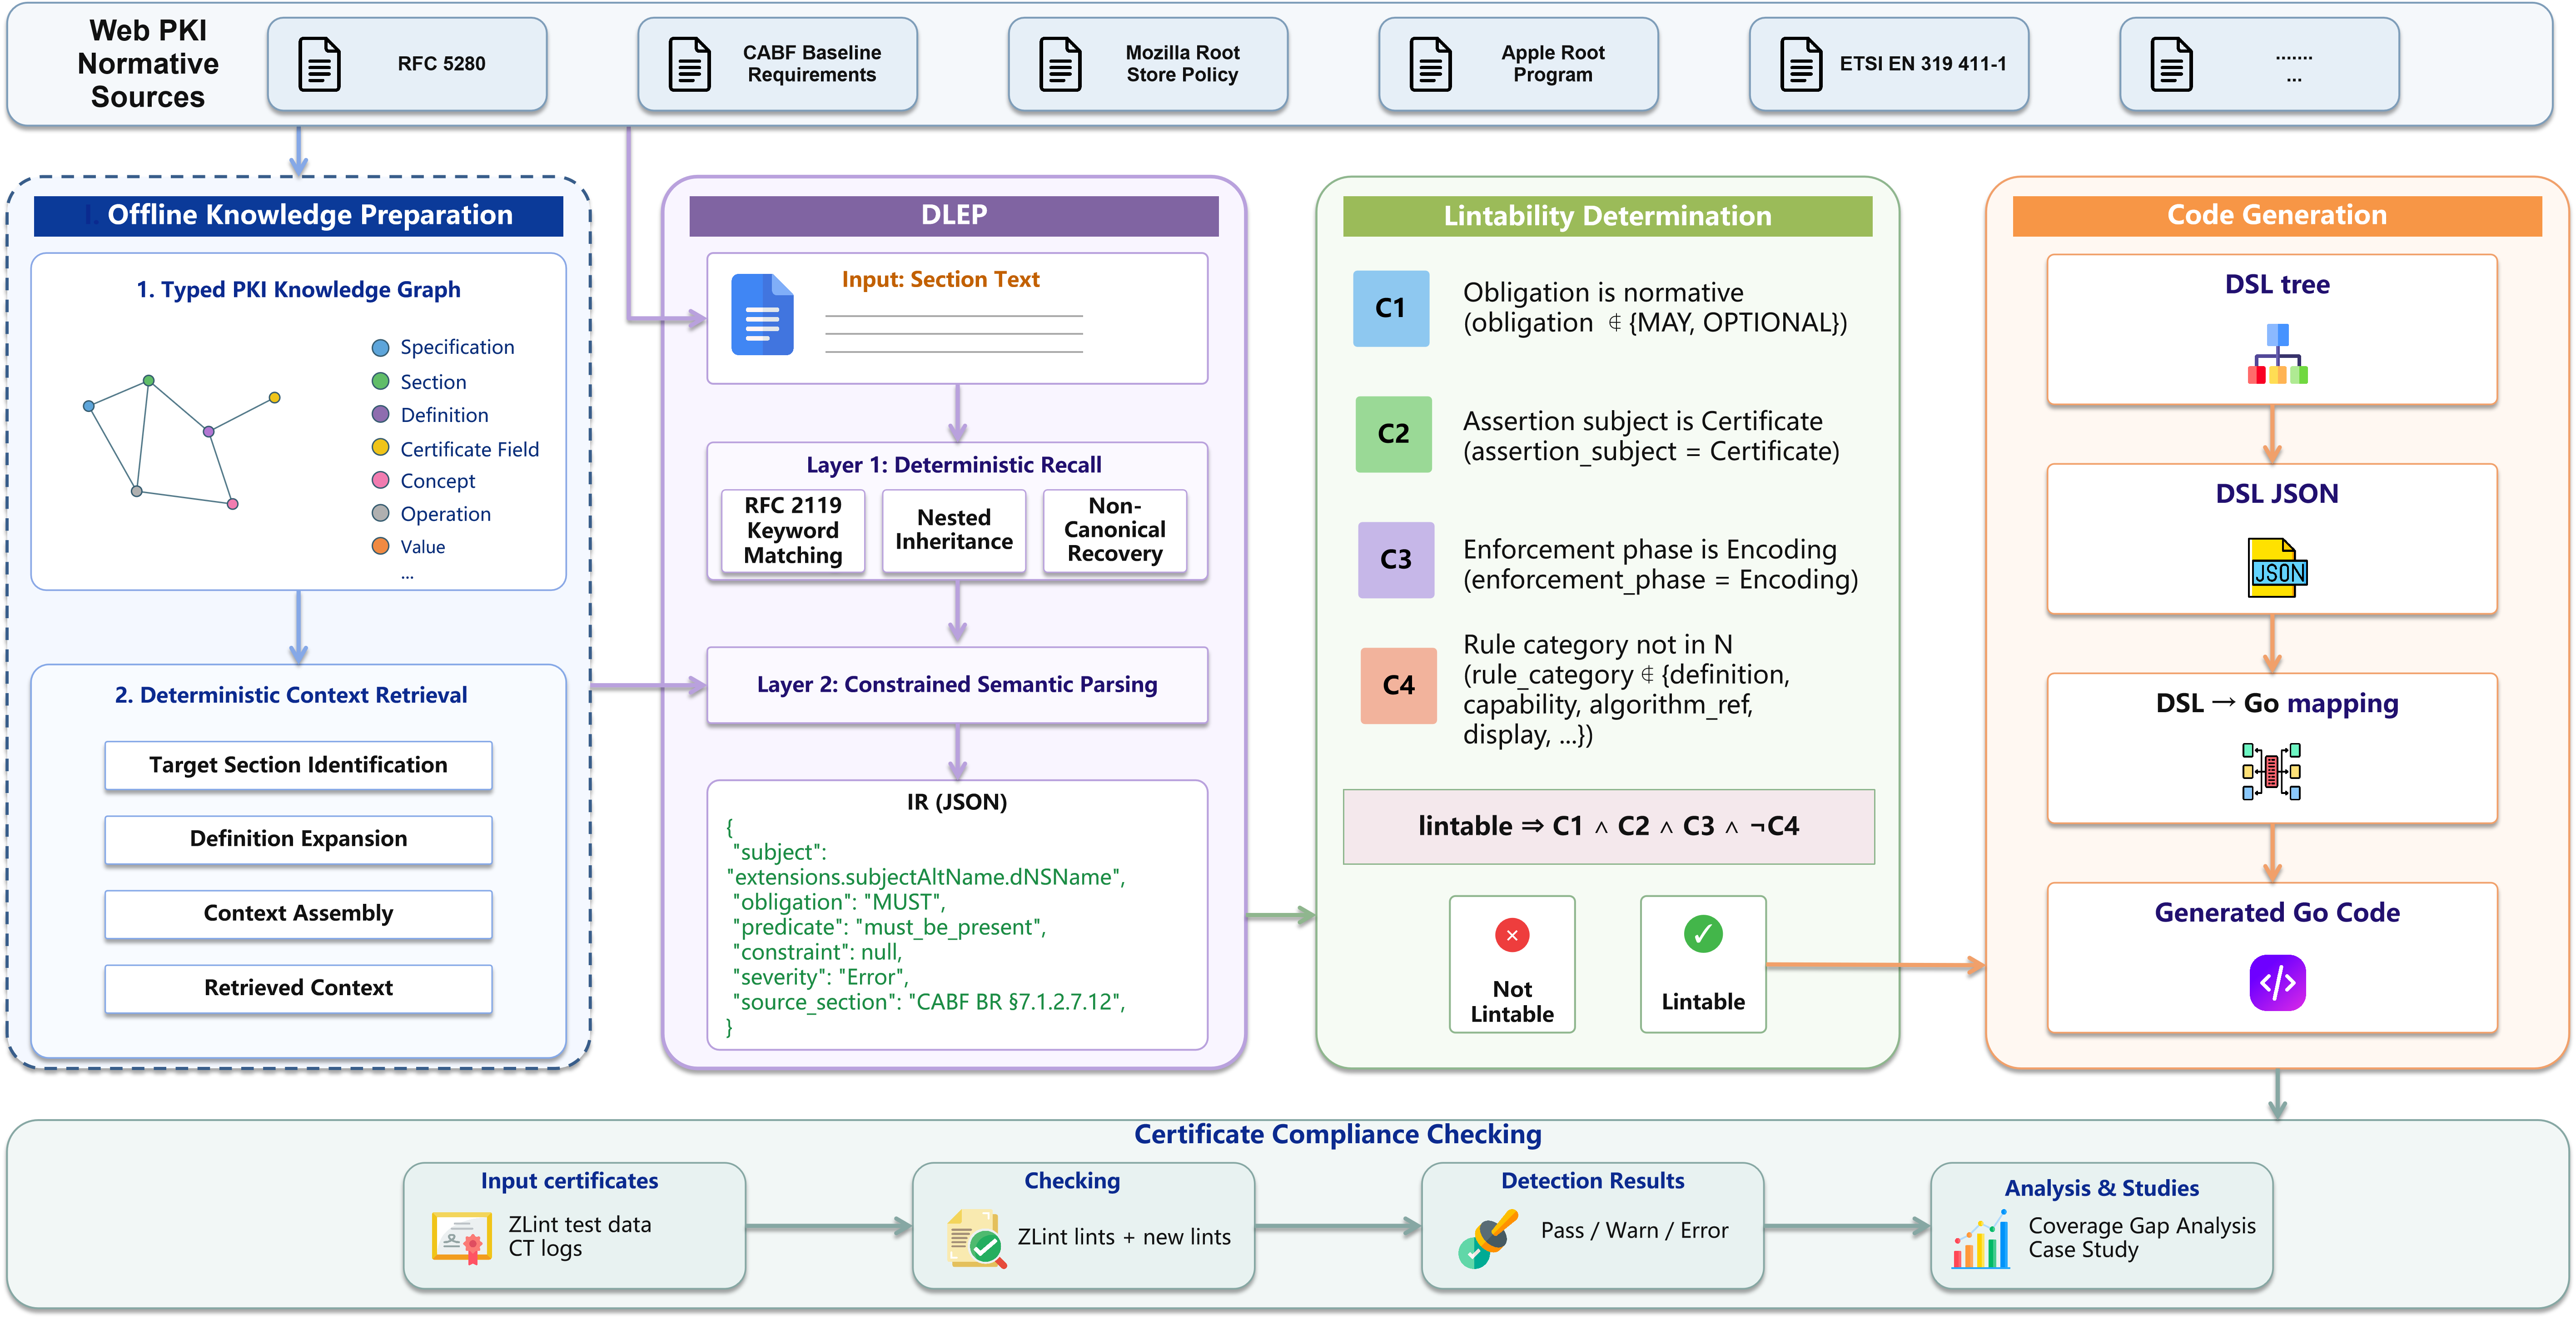
\includegraphics[width=\textwidth]{figures/fig01_architecture.png}
  \caption{Overall Architecture of the Framework.}
  \Description{Four-module architecture connecting Web PKI sources, deterministic context retrieval, normative-rule extraction, and restricted lint generation.}
  \label{fig:architecture}
\end{figure*}

%-------------------------------------------------------------------------------
\section{Normative Rule Extraction}
\label{sec:rule-extraction}
%-------------------------------------------------------------------------------

This section presents our methodology for extracting normative rules from Web
PKI normative sources and converting them into a structured IR.

\subsection{PKI Knowledge Graph Builder}
\label{sec:method-kg-builder}

The PKI knowledge graph builder is the offline component that converts heterogeneous Web PKI normative sources into the retrieval substrate.
It normalizes each normative source into a hierarchical structure with stable identifiers for the source, sections, headings, and text units.
It then extracts explicit references such as section citations, RFC references, and policy cross-links, and links them to target nodes when the targets can be resolved unambiguously.
In parallel, it records certificate-field concepts and aliases such as subjectAltName, dNSName, basicConstraints.cA, and policy OIDs, to map natural-language mentions to canonical certificate paths during later extraction.

Web PKI normative sources form a densely interconnected cross-document network.
For example, RFC~5280 references multiple RFCs, while CABF~BR directly depends on RFC~5280 field definitions.
We model this knowledge as a multi-edge directed graph. Its eight node types are Specification, Section, Definition, CertificateField, Rule, Operation, Value, and Concept, and its four source-backed relations are CONTAINS, DEFINES, REFERENCES, and APPLIES\_TO. Appendix~\ref{app:kg} summarizes these relations and their deterministic retrieval constraints.

This builder is deliberately conservative.
It stores only relations directly supported by source-document structure or textual evidence, while leaving normative judgments such as conflict, override, and lintability to later deterministic stages.
Normative-judgment relations such as CONFLICTS\_WITH and OVERRIDES are produced independently by the rule engine and are not included in the retrieval graph.
The resulting graph serves as a traceable context index rather than as an oracle. It helps the extractor identify definitions, inherited constraints, and referenced normative rules, but does not determine whether a normative rule is lintable.

\subsection{Deterministic Context Retrieval}
\label{sec:method-graphrag}

To address cross-document references, We organize context deterministically rather than relying on the LLM to infer relations.
We implement a deterministic retrieval module based on GraphRAG~\cite{edge2024local} that treats the knowledge graph of \S\ref{sec:method-kg-builder} as a fixed input and retrieves context through bounded subgraph queries.

Given a target Section node, the retrieval module performs a BFS expansion over the $k$-hop neighborhood using the source-backed CONTAINS, DEFINES, REFERENCES, and APPLIES\_TO relations.
It then assembles LLM context by relation-type priority and provides term definitions, field metadata, and referenced sections. The retrieval process uses neither vector similarity nor LLM inference, and produces no independent judgment.

\subsection{DLEP}
\label{sec:method-dual-layer}

\begin{table}[!htbp]
\centering
\caption{RFC~2119 keyword tiers.}
\label{tab:rfc2119}
\setlength{\tabcolsep}{4pt}
\footnotesize
\begin{tabularx}{\columnwidth}{@{}L{0.27\linewidth} L{0.30\linewidth} X@{}}
\toprule
Tier & Keywords & Semantics \\
\midrule
Mandatory      & MUST, SHALL, REQUIRED   & Absolute requirement; a violation is non-compliance \\
Prohibition    & MUST NOT, SHALL NOT     & Absolute prohibition \\
Recommendation & SHOULD, SHOULD NOT, RECOMMENDED & Strongly recommended or discouraged; justified deviation permitted \\
Optional       & MAY, OPTIONAL           & Fully optional \\
\bottomrule
\end{tabularx}
\end{table}

\begin{table}[!htbp]
\centering
\caption{IR core four-tuple fields.}
\label{tab:ir-core}
\setlength{\tabcolsep}{4pt}
\footnotesize
\begin{tabularx}{\columnwidth}{@{}L{0.18\linewidth} X@{}}
\toprule
Field & Meaning \\
\midrule
subject    & Certificate field path, for example extensions.\allowbreak subjectAltName.\allowbreak dNSName, resolved by FieldResolver \\
obligation & RFC~2119 keyword, such as MUST/SHALL/SHOULD/\dots \\
predicate  & Assertion type, such as must\_be\_present, conform\_to, equal, \dots \\
constraint & constraint value or pattern \\
\bottomrule
\end{tabularx}
\end{table}

To limit the role of the LLM in extraction, we design DLEP as a dual-layer pipeline that separates deterministic normative-rule recall from schema-constrained semantic parsing.

Layer~1 performs deterministic normative-rule recall.
Web PKI normative sources commonly express normative rules using the RFC~2119 keywords listed in Table~\ref{tab:rfc2119}.
RFC~8174 further specifies that these keywords carry normative force only when capitalized, enabling deterministic keyword matching.

To maximize recall, Layer~1 operates in three passes.
Pass~1 directly matches RFC~2119 keywords.
Pass~2 detects nested structures so subordinate normative rules inherit the parent obligation level.
Pass~3 performs Non-Canonical Recovery.

Layer~2 performs controlled semantic parsing using an LLM, but restricts the model to a constrained language-understanding role.
Instead of generating lint rules or compliance judgments directly, Layer~2 converts normative text into a JSON-serialized IR, while all normative reasoning is deferred to later deterministic stages.

\begingroup\emergencystretch=2em\relax
The IR decouples semantic extraction from downstream tasks, allowing the same extraction result to support multiple uses, as shown in Fig.~\ref{fig:ir-downstream}.
Each IR record is serialized as a JSON object with 33 fields.
Its core component, shown in Table~\ref{tab:ir-core}, is the four-tuple
$\mathrm{IR} = \langle\text{subject}, \text{obligation}, \text{predicate}, \text{constraint}\rangle$,
together with 29 extension fields summarized in Appendix~\ref{app:ir}.
\par\endgroup


The IR design provides three properties used by downstream stages.
First, citation, constraint, and obligation information are stored separately, supporting traceability and conflict handling.
Second, the IR serves as the fixed input to the four-condition lintability determination in \S\ref{sec:method-lintability}, making that determination deterministic for a given IR.
Third, once a normative rule is determined to be lintable, field paths, assertion types, and constraint values are explicit inputs to DSL-tree synthesis and inspection.

To constrain LLM behavior, Layer~2 enforces a predefined schema and category set.
Every extracted normative rule must map to explicit source text, and certificate field hierarchies must follow the ASN.1 path definitions in RFC~5280.
The IR generation process is also staged. The model first determines the normative-rule category and then fills in the remaining fields.
Appendix~\ref{app:ir} provides the category definitions, correction rules, and tuning details.

\begin{figure}[!htbp]
  \centering
  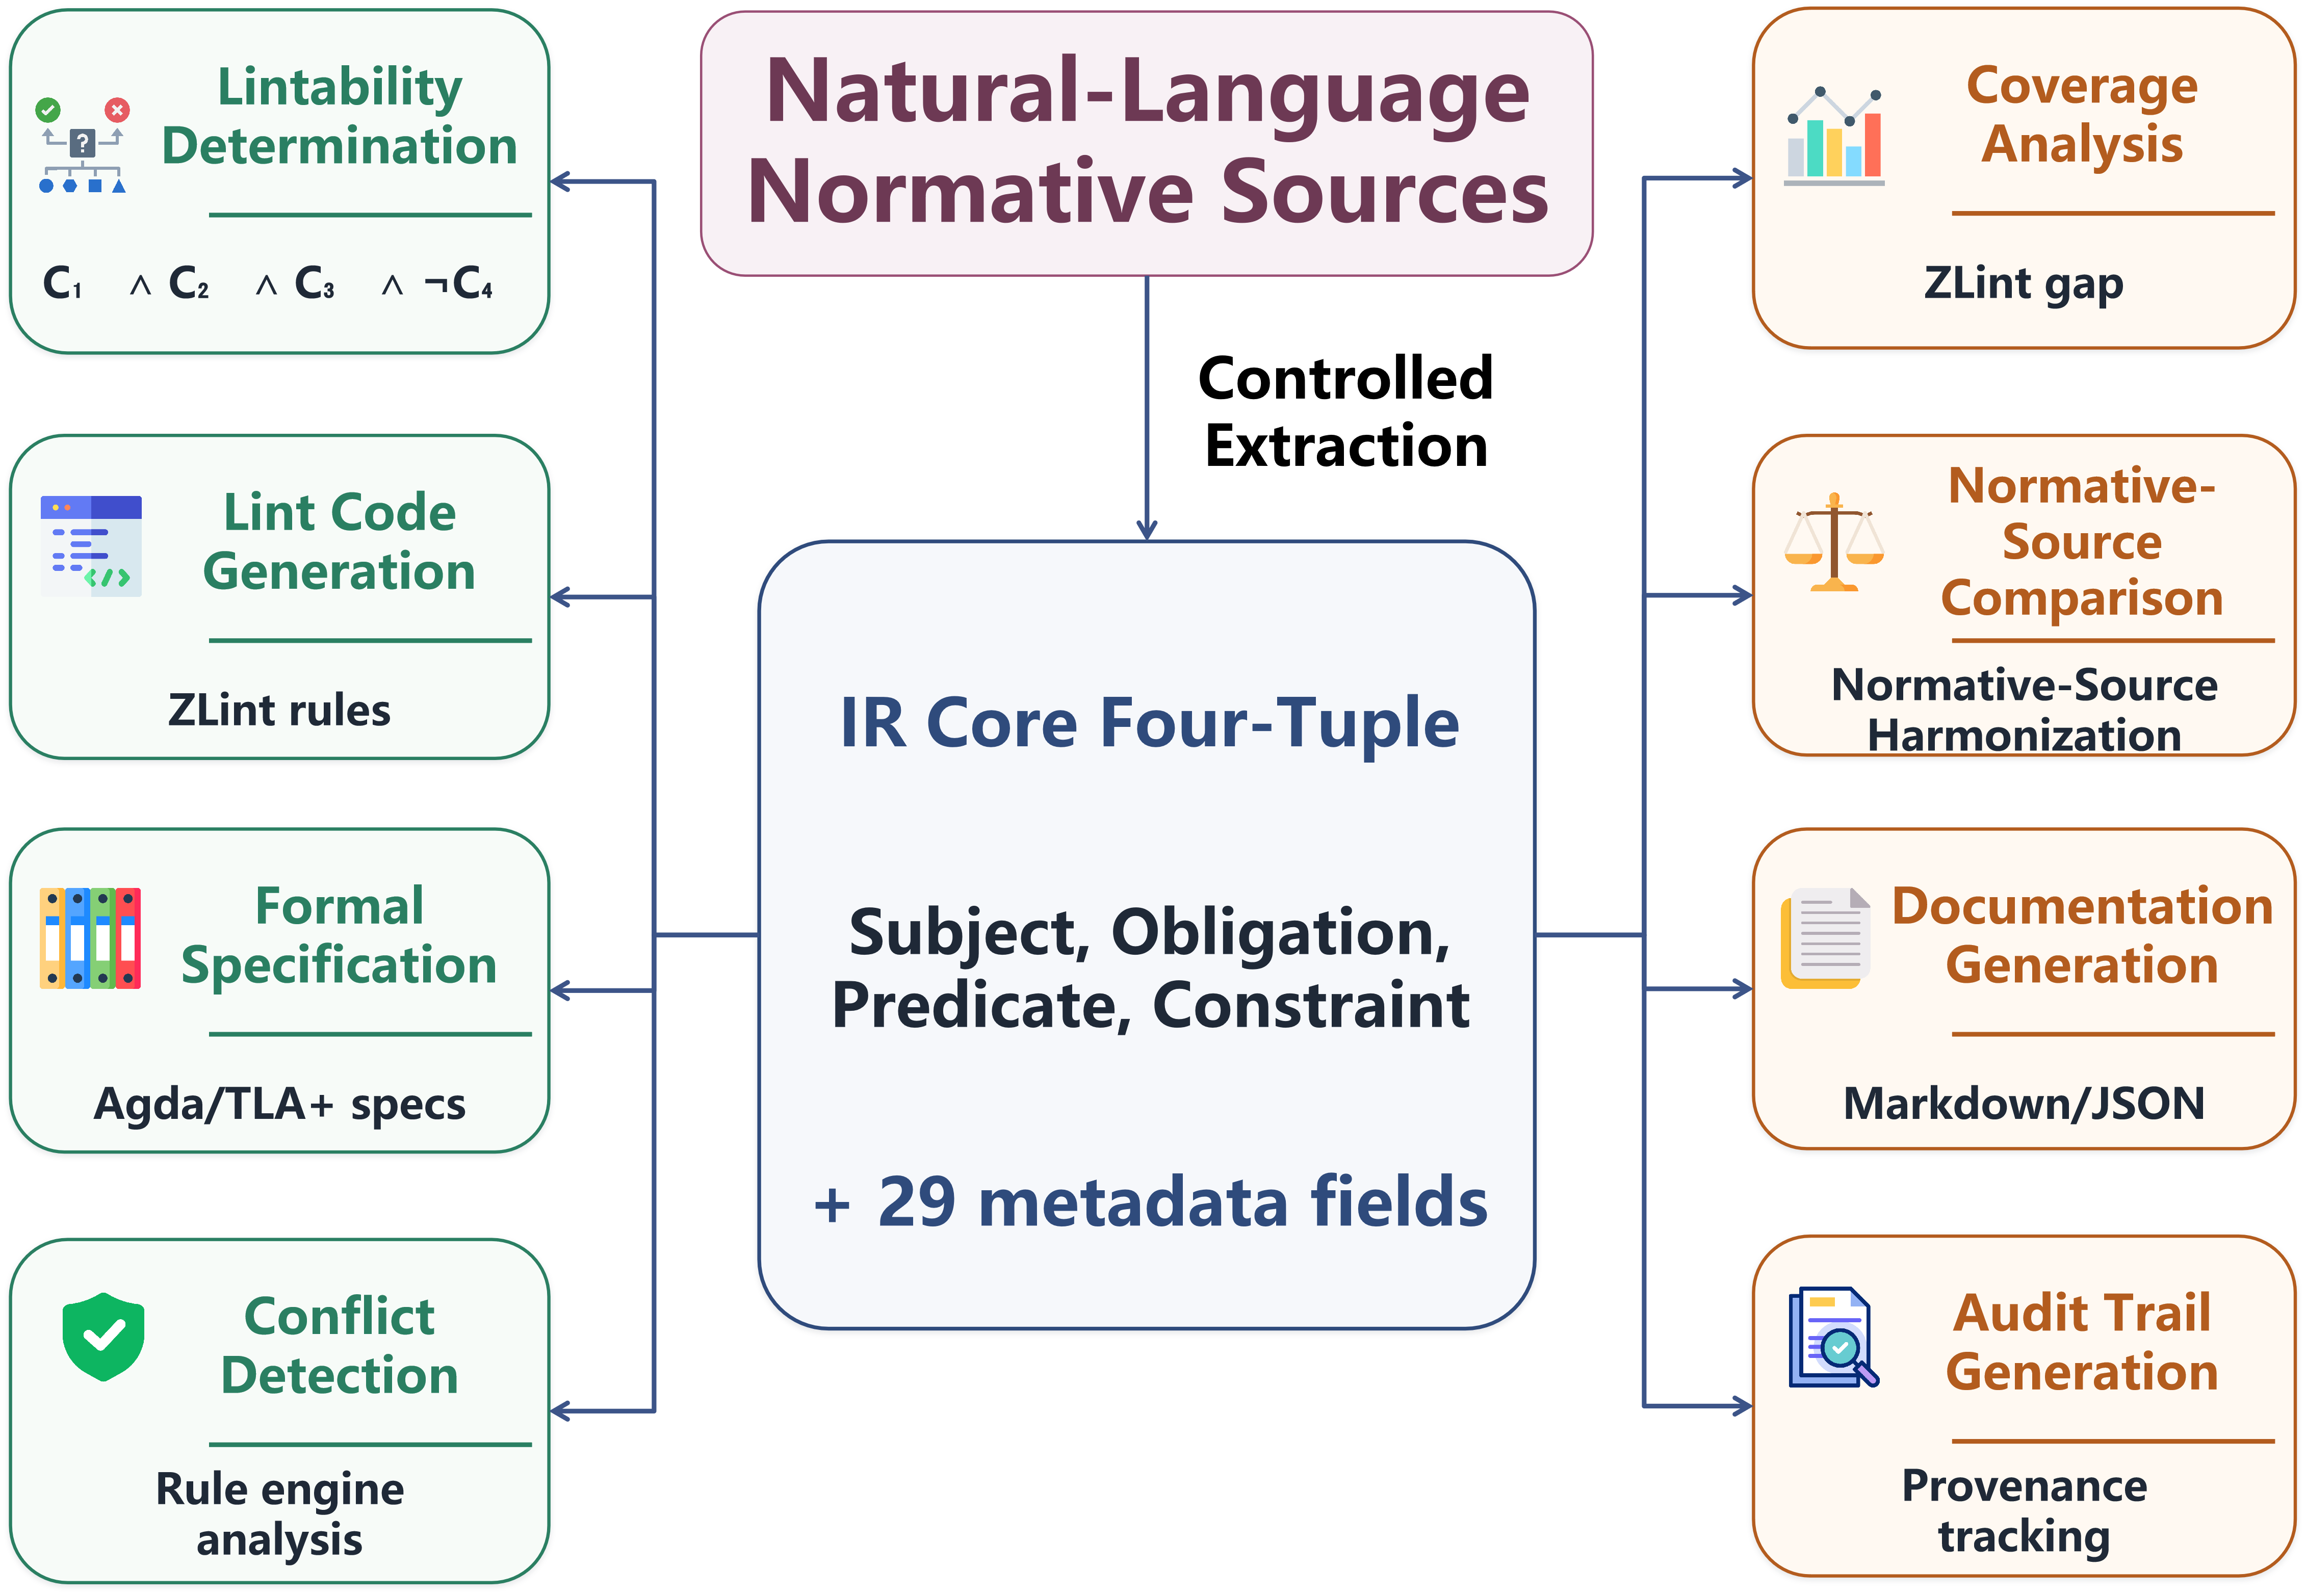
\includegraphics[width=\linewidth]{figures/fig02_ir_downstream.png}
  \caption{IR-driven architecture in which a single extraction pass feeds every
    downstream stage.}
  \Description{A structured intermediate representation flows from normative text extraction to lintability analysis, code generation, and validation.}
  \label{fig:ir-downstream}
\end{figure}

%-------------------------------------------------------------------------------
\section{Lintability Determination}
\label{sec:method-lintability}
\label{sec:lintability}
%-------------------------------------------------------------------------------

\begin{table*}[tb]
\centering
\caption{The four lintability conditions, each a Boolean function of one IR field.}
\label{tab:four-conditions}
\footnotesize
\setlength{\tabcolsep}{4pt}
\begin{tabularx}{\textwidth}{@{}l l L{0.36\linewidth} X@{}}
\toprule
ID & IR field & Value domain & Condition \\
\midrule
$C_1$      & obligation         & MUST, SHALL, REQUIRED, SHOULD, RECOMMENDED, MUST NOT, SHALL NOT, SHOULD NOT, MAY, OPTIONAL & obligation $\notin$ \{MAY, OPTIONAL\} \\
$C_2$      & assertion\_subject & Certificate, CA, CrossArtifact & assertion\_subject $=$ Certificate \\
$C_3$      & enforcement\_phase & Encoding, Validation, Comparison, Processing & enforcement\_phase $=$ Encoding \\
$\neg C_4$ & rule\_category     & encoding\_constraint, comparison, definition, capability, algorithm\_ref, display, \dots & rule\_category $\notin$ \{definition, capability, algorithm\_ref, display, \dots\} \\
\bottomrule
\end{tabularx}
\end{table*}

Before generating code, we determine the lintability of each normative rule, namely
whether it admits such a certificate lint. Rather than asking the LLM to make
this judgment directly, we compute it from the IR that the LLM has already
produced. Three observations motivate this design. First, our operational
criterion uses four pieces of information, namely the deontic strength of the
obligation, who is obligated, when the obligation applies, and what type of normative rule
it is. Second, each of the four can be encoded as
a single IR field with a small, closed value set, so the LLM performs a
lower-entropy selection of each field value from the enumerated Value domain
column of Table~\ref{tab:four-conditions}. The lintability
determination then becomes a Boolean function of four discrete fields. Third,
separating the four conditions makes the IR fields contributing to a label
explicit rather than locating the determination in an opaque end-to-end LLM call.

Table~\ref{tab:four-conditions} lists the four IR fields, their value domains, and the conditions they determine. The deontic level obligation comes from the IR core four-tuple in Table~\ref{tab:ir-core}. The remaining three key extension fields are assertion\_\allowbreak subject, enforcement\_\allowbreak phase, and rule\_\allowbreak category. From the enumeration of rule\_\allowbreak category, we designate
\begin{gather*}
\mathcal{N} = \{definition,\,capability,\,algorithm\_ref,\,display,\,\dots\}
\end{gather*}
as the subset whose normative-rule type carries no certificate lint over the certificate. This subset covers term definitions, CA capability statements, delegations to external algorithm specifications, UI rendering rules, and similar non-encoding rule types.

The four conditions in Table~\ref{tab:four-conditions} are necessary for lintability, and each is a Boolean function of exactly one IR field:
\begin{equation}\label{eq:lintable}
\mathrm{lintable}(r) \;\Longrightarrow\; C_1(r)\wedge C_2(r)\wedge C_3(r)\wedge \neg C_4(r),
\end{equation}
\begin{align*}
C_1(r) &\equiv \mathrm{is\_normative}(r.\text{obligation}), \\
C_2(r) &\equiv r.\text{assertion\_subject} = Certificate, \\
C_3(r) &\equiv r.\text{enforcement\_phase} = Encoding, \\
C_4(r) &\equiv r.\text{rule\_category} \in \mathcal{N}.
\end{align*}
The obligation field also fixes the lint severity. MUST-class obligations map to Error, and SHOULD-class obligations map to Warning. Severity is therefore not a second determination function, but a direct read of obligation.

The three non-deontic conditions encode three orthogonal boundaries. $C_2$ is the subject boundary, separating obligations on the certificate from obligations on the CA, relying party, or surrounding ecosystem. $C_3$ is the runtime boundary, separating obligations observable in the issued bytes from those that fire during chain processing, name comparison, revocation handling, or CAA retrieval. $\neg C_4$ is the process boundary, separating state assertions from terms in $\mathcal{N}$.

Since each $C_i$ is a deterministic function of one IR field, the lintability
determination, which adopts the conjunction $C_1\wedge C_2\wedge C_3\wedge\neg C_4$ of
these necessary conditions as its operational criterion, is computed from
the IR rather than predicted by the LLM. When the values of the four IR fields
used by this criterion are fixed, repeated evaluation yields the same
lintability result.

%-------------------------------------------------------------------------------
\section{Restricted Code Generation}
\label{sec:codegen}
%-------------------------------------------------------------------------------

Generating checking code directly with an LLM faces two
inherent difficulties. The first is hallucination. The model may
misspell a field name as another field that happens to exist but is
semantically unrelated, or introduce a unit error in an OID. The second is
output instability. The same code-generation prompt often produces
different outputs across calls, with no guarantee that the result will compile or
be logically correct. To contain this uncertainty, we confine a rule's code body
to a finite, closed DSL-tree space $\Tv$. Each rule's code body can only be a
tree in that space, which is then rendered into Go code by a deterministic
function. The deterministic main path avoids unconstrained code emission, and
the restricted LLM fallback is bounded to the same closed space and gated by
``render and pass go build,'' so any out-of-space or non-compiling output is
rejected rather than shipped.
Figure~\ref{fig:codegen-pipeline} illustrates the whole
pipeline on a single normative rule: CA certificates must assert the keyCertSign
key-usage bit.

\begin{figure*}[tb]
  \centering
  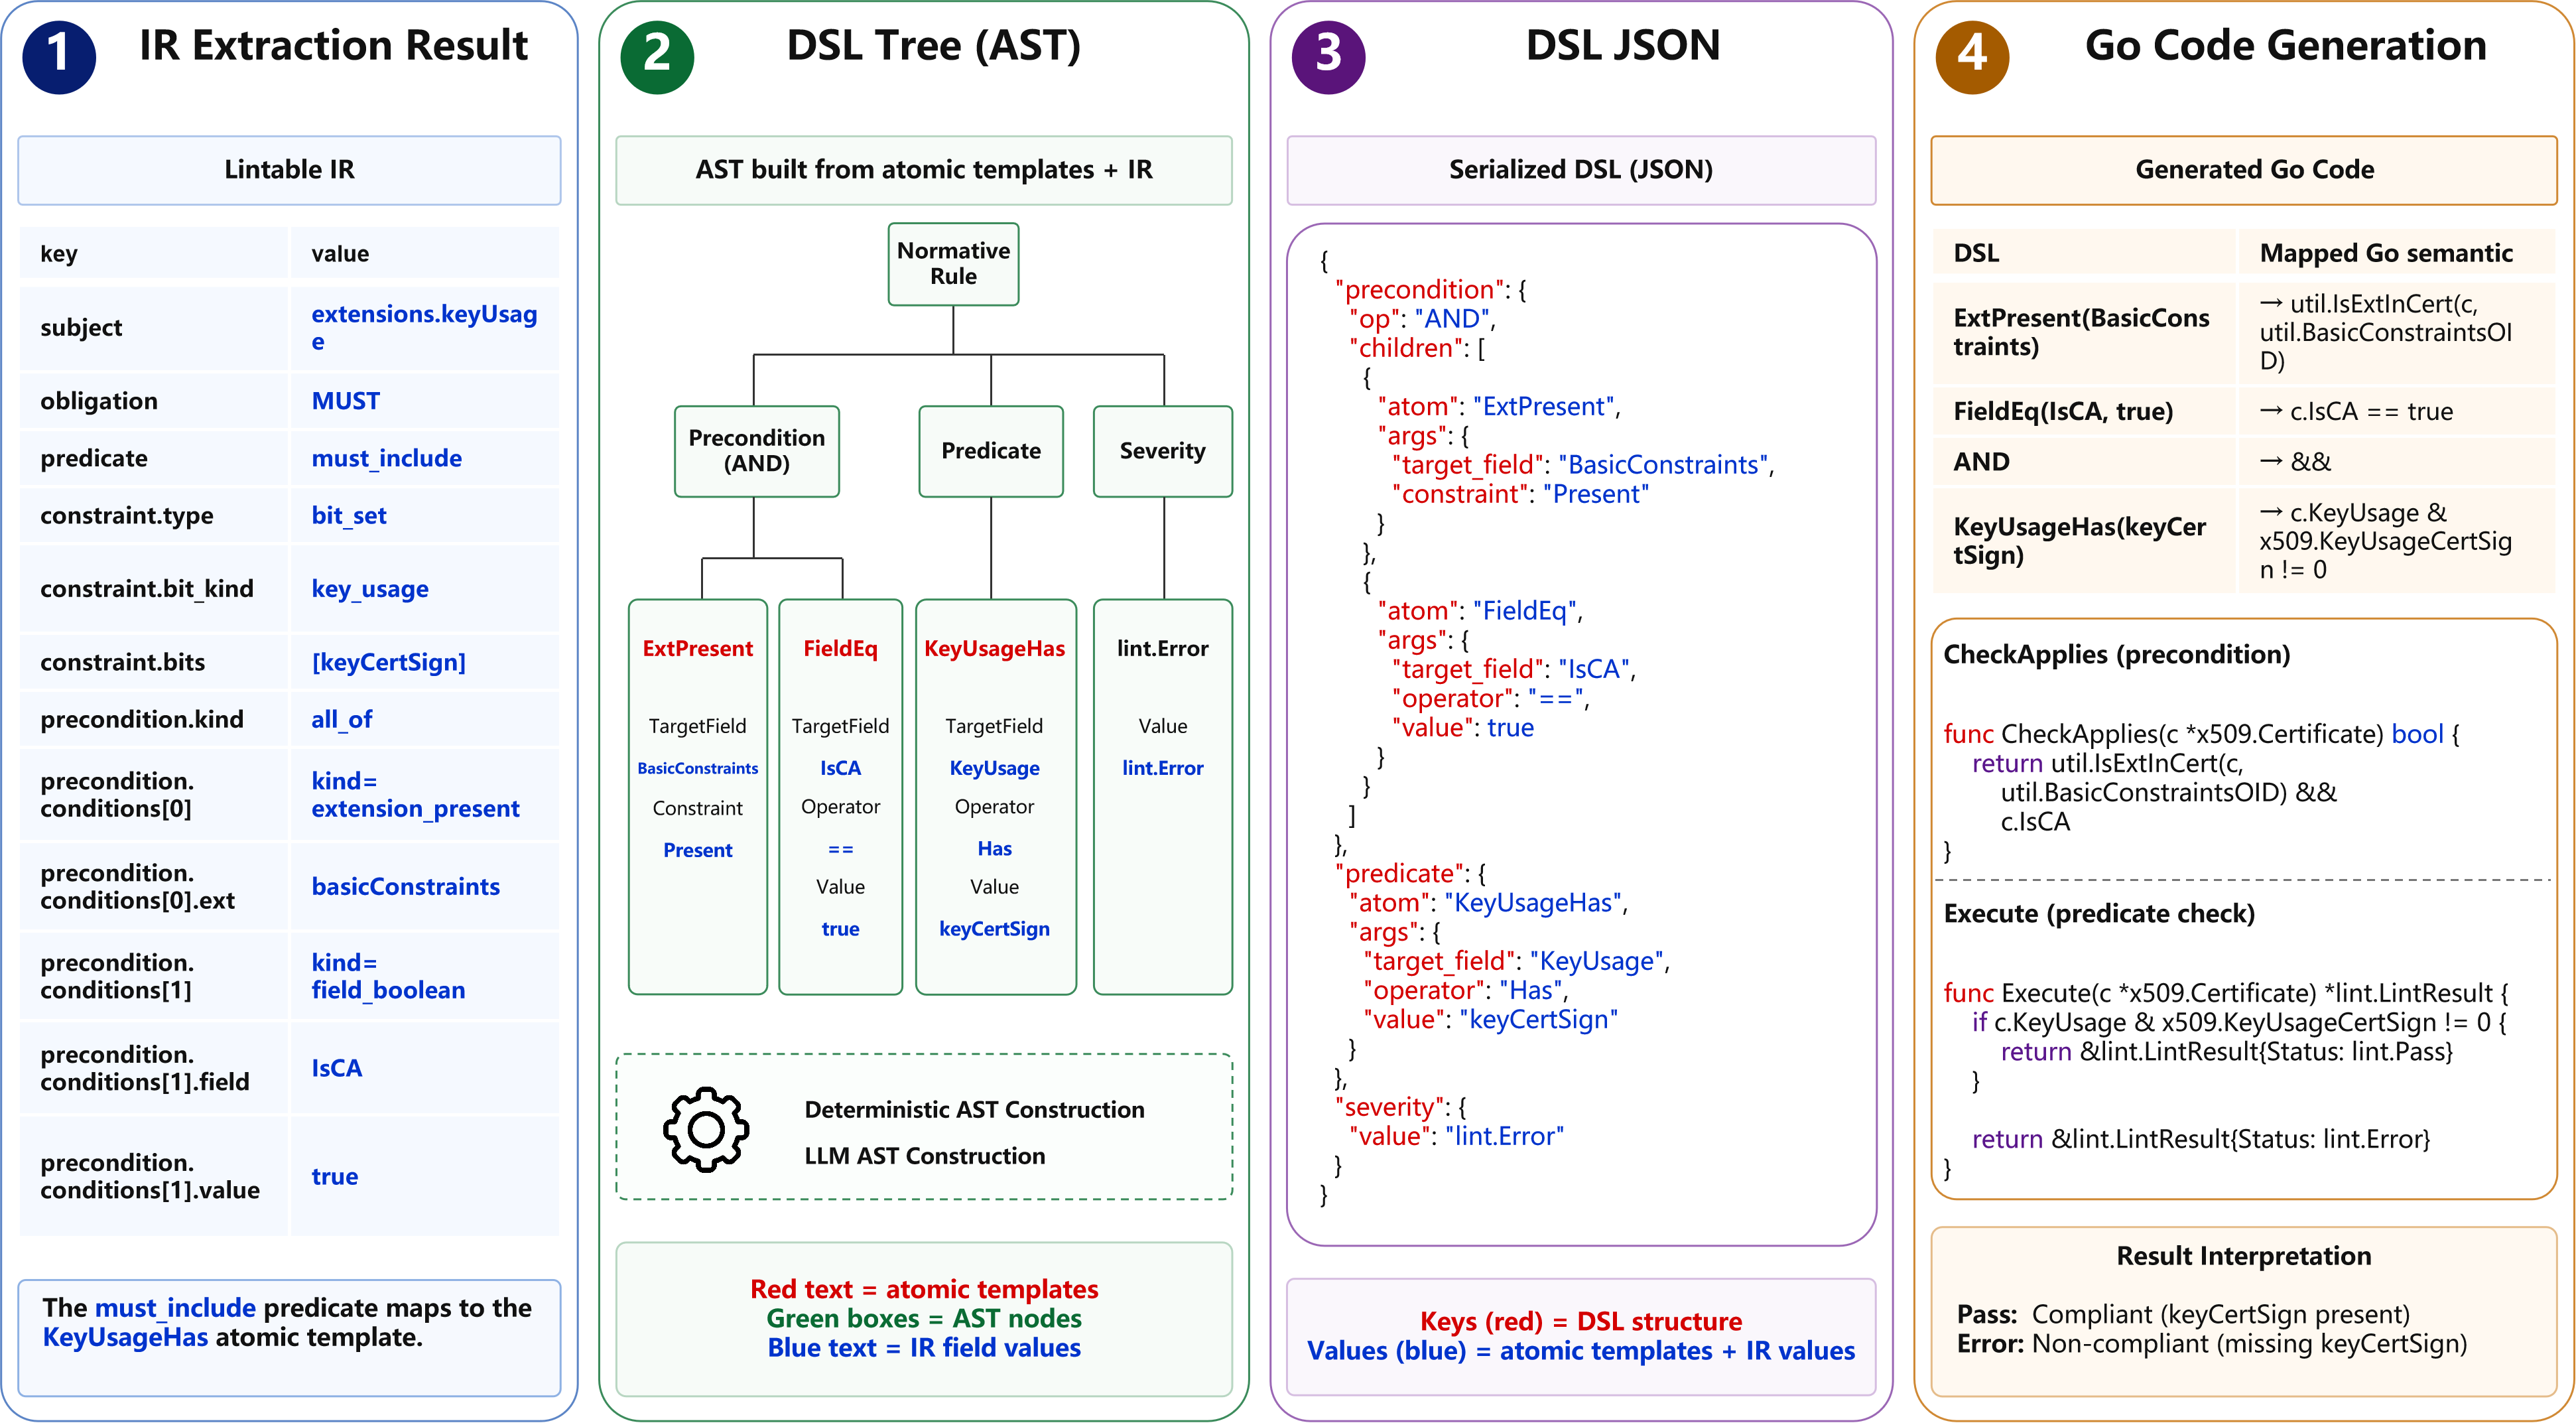
\includegraphics[width=\textwidth]{figures/fig03_codegen_pipeline.png}
  \caption{Worked example of restricted code generation. }
  \Description{A worked pipeline example shows a normative key-usage rule becoming an IR record, a restricted DSL tree, and rendered checking code.}
  \label{fig:codegen-pipeline}
\end{figure*}

\subsection{Atomic Templates and IR Filling}
\label{subsec:atoms}

An atomic template is the smallest unit of a certificate lint.
Most certificate lints in PKI are logical combinations of a
few atomic templates that test whether an extension is present, whether a
field equals a constant, or whether every element of a list matches a
pattern, and combining such atomic templates with conjunction, disjunction, and
negation can
characterize most static constraints. The abstract syntax of the code DSL is:
\begin{equation}\label{eq:grammar}
  \mathcal{T} \;::=\; a(\bar{v}) \;\mid\; \neg\, \mathcal{T} \;\mid\;
  \mathcal{T} \wedge \mathcal{T} \;\mid\; \mathcal{T} \vee \mathcal{T}
\end{equation}
where $a \in \mathcal{A}$ is an atomic-template predicate and $\bar{v}$ is its
argument list. $\mathcal{A}$ is a finite, closed set of atomic
templates, and $\{\neg, \wedge, \vee\}$ are
the propositional-logic combinators.

\textbf{Generality grading, GENERIC and SPECIALIZED.} Atomic templates are
graded by semantic reuse. An atomic template is GENERIC if it expresses a
general PKI certificate-attribute judgment reusable across normative rules and
is not tied to a corpus-specific OID, a single clause, or a one-off extension
structure, as $\mathrm{ExtPresent}$ is; otherwise it is SPECIALIZED, as
$\mathrm{DomainComponentOrdered}$ is, which checks only the RFC~4519 ordering of
a Subject DN's domainComponent. The grading is fixed in code as two sets with a
partition-completeness assertion and is deterministically recomputable. The
the current implementation has 183 atomic templates, 118 GENERIC and 65 SPECIALIZED, with
representative members in Appendix~\ref{app:tv}. The code body of a lint rule is modeled as
an ordered pair $(p, q) \in \mathcal{T}_\varepsilon \times \mathcal{T}$, where
$q \in \mathcal{T}$ is the main assertion and $p \in \mathcal{T}_\varepsilon =
\mathcal{T} \cup \{\varepsilon\}$ is an optional precondition, where $\varepsilon$
marks an absent precondition. In the
equation below, $c$ is a single certificate, and $\lVert u \rVert(c) \in
\{\mathrm{true}, \mathrm{false}\}$ denotes the Boolean result of evaluating a
DSL tree or precondition $u$ on $c$; atomic templates evaluate by their semantics, and
$\neg/\wedge/\vee$ by classical propositional logic. The execution semantics
is:
\begin{equation}\label{eq:exec}
  \lVert (p, q) \rVert(c) \;=\;
  \begin{cases}
    \mathrm{NA}, & p \neq \varepsilon \,\land\, \lnot\lVert p \rVert(c) \\[2pt]
    \mathrm{Pass}, & (p = \varepsilon \,\lor\, \lVert p \rVert(c)) \,\land\,
      \lVert q \rVert(c) \\[2pt]
    \mathrm{Severity}(r), & \text{otherwise}
  \end{cases}
\end{equation}
The precondition $p$ is the normative rule's precondition. When it exists and is
false on $c$, the result is $\mathrm{NA}$, meaning not applicable; when the
precondition is absent or holds and $q$ holds, the result is $\mathrm{Pass}$;
when the precondition holds but $q$ does not, it is a violation, returning
$\mathrm{Severity}(r)$ by obligation. Because $C_1$ of \S\ref{sec:lintability}
already excludes MAY/OPTIONAL, an obligation entering generation must be
MUST-class or SHOULD-class, so $\mathrm{Severity}(r) \in \{\mathrm{Error},
\mathrm{Warn}\}$.

\textbf{The IR fills the atomic template's parameter slots.} Selecting an atomic
template fixes only which check to use; one still needs to know what to check and
against what value, and these parameter values come precisely from the current
normative rule's IR. The IR's subject is the certificate field path given by the
field resolver, such as subjectAltName.dNSName, and it fills the atomic
template's field slot. The IR's constraint is a constraint value or
pattern such as a value set, a length interval, or a regex name, and it fills the value
slot. For example, the normative rule ``the dNSName of subjectAltName must be non-empty''
is, after mapping and filling, instantiated as
$\mathrm{FieldNonEmpty}(\mathrm{DNSNames})$.

\textbf{Mapping IR predicates to atomic templates.} The upstream
IR and the downstream DSL use two vocabularies. The IR describes normative rules
with extraction-stage predicates such as must\_be\_present,
encode\_as, and in\_range, while the DSL expresses checks with
atomic templates, and the two are not in one-to-one correspondence. To
bridge them, we maintain a many-to-many predicate-to-template map that assigns each IR
predicate a set of candidate atomic templates that can semantically carry it.
For instance, must\_be\_present may correspond to $\{\mathrm{ExtPresent},
\mathrm{FieldNonEmpty}\}$, and in\_range to $\{\mathrm{IntInRange},
\mathrm{PathLenConstraintHas}, \dots\}$. Which one to take depends on the type
of the constrained field.

\subsection{Typed Vocabulary and Parameter Closure}
\label{subsec:tv}

\S\ref{subsec:atoms} described how atomic templates and IR filling place the
IR's subject and constraint into an atomic template's parameter slots, but the
IR provides only the field that a normative rule restricts and the value it
restricts that field to,
without constraining the legal type of those values. If the subject path
in the IR points to a nonexistent field, or a string is placed into a slot that
requires an integer, a structurally legal but semantically misaligned tree can
still result. This subsection closes that gap with a typed vocabulary
$\mathcal{V}$. $\mathcal{V}$ is the disjoint union of seven finite sets, frozen
at system startup, and each atomic-template parameter may only draw from one of
them: certificate field names, DN fields, OID constants, KeyUsage bits,
ExtKeyUsage bits, ASN.1 encoding types, and named regexes. The size and samples
of each class appear in Appendix~\ref{app:tv}.

\begingroup\emergencystretch=2em\relax
Each atomic template has a signature table that specifies, for each parameter,
which class or base type integer/Boolean/string it must draw from; a call to an
atomic template is legal if and only if every actual argument falls in the class its
signature prescribes. Writing $\Tv$ for the set of DSL trees all of whose
parameters are legal, we strictly restrict the range of the code generator to
it. Any tree in $\Tv$ contains no field name, OID, or regex
outside $\mathcal{V}$; an out-of-bounds tree necessarily errors at the parsing
stage, triggering repair, and never enters code generation.
\par\endgroup


\subsection{Code Generation and Mechanical Translation}
\label{subsec:mech}

A legal DSL tree $t$ must be turned into two products. One is executable Go
checking code, and the other is a code summary that
summarizes its checking logic in one sentence. Both conversions are performed by
deterministic total functions, with no LLM call. The rendering function $\rho$
maps a tree to Go code, and the mechanical translation function $\smech$, read as
the mechanical summarizer, maps the
same tree to a code summary sentence; for the same $t$, each produces a unique
output. Informally, $\rho(t)$ is what the checker runs and $\smech(t)$ is what it
says it runs; both being fixed functions of $t$, the second cannot flatter the
first.

$\rho$ is type-safe. It never generates an out-of-bounds field, OID, or
parameter type, so closure is preserved from the DSL-tree layer down to the
Go-code layer. Together with determinism, this makes $\rho(t)$ a fixed function
of $t$.
$\smech$, by contrast, is structure-preserving. Each atomic template and
combinator maps to a distinct phrase, so $\smech(t)$ retains the structural
information of the DSL tree in the verification chain; the construction is
detailed in Appendix~\ref{app:sigma}.

\begingroup\emergencystretch=2em\relax
Thus $\rho$'s product leads to executable code, while $\smech$'s product leads to
semantic-equivalence verification, which compares the code summary with the
normative rule text and determines whether the two are semantically equivalent.
\par\endgroup


\subsection{Tree Synthesis with a Deterministic Main Path and Restricted LLM
Fallback}
\label{subsec:synth}

The preceding discussion described how the IR filling of \S\ref{subsec:atoms} and the
parameter closure of \S\ref{subsec:tv} confine a DSL tree to $\Tv$, but two
decisions still require synthesis. The first is which atomic template carries
which IR predicate. The second is whether the IR's subject and
constraint can both be filled into the chosen atomic template.
This subsection gives the implementation of the generator. It
first attempts deterministic synthesis and falls back to LLM synthesis only when
deterministic synthesis returns no tree. Both paths use rendering and passing go build as
the acceptance gate. Even if deterministic synthesis returns a tree, that is
not enough; it must actually compile, otherwise it is treated as unresolved and
passed to LLM synthesis. Both paths are constrained by the same set of
structural checks; they only confine the output to a traceable space.

\textbf{Deterministic main path.} When an IR predicate selects an atomic
template through the predicate-to-template map and its subject and constraint can fill that template's
parameter slots, the generator deterministically derives a DSL tree using
predefined rules. Here, deriving means constructing a DSL tree from the IR step by
step by fixed rules, with no LLM call throughout. Most lintable normative rules in our
study are covered by this deterministic path.

\textbf{Restricted LLM synthesis.} When deterministic synthesis returns no tree,
the generator switches to LLM synthesis. The model receives the normative-rule context,
the structured IR, the candidate atomic-template set, and a readable enumeration
and signature table of $\mathcal{V}$ and $\mathcal{A}$. It
outputs only one of two results, either a serialized DSL tree or an explicit
no-template abstention marker (NT). The raw LLM
output is first validated by a parser, which resolves it into
a legal DSL tree $t \in \Tv$, a type error, or NT, and any
identifier outside $\mathcal{V}/\mathcal{A}$ is rejected here; a passing tree is
rendered by $\rho$, and then a deterministic post-processor
binds the lint's metadata, taking Description from the IR's rule\_text field,
which holds the verbatim text of the normative rule, Citation from the source
identifier and section number, and Name from the DSL tree and the rule
identifier, with details in Appendix~\ref{app:tv}.

\subsection{Manual Semantic Alignment Verification}

Whether the generated code expresses the normative rule is the hardest judgment
in the whole pipeline and requires manual review because the normative sentence
is expressed partly in prose.

\noindent\textbf{Description provenance.}\par\noindent Description is an IR field. When Layer~2 of DLEP parses a normative sentence, it stores that
sentence verbatim in the IR's rule\_text field, and the deterministic
post-processor of \S\ref{subsec:synth} copies that field unchanged into the
Description metadata of every generated lint, on both the deterministic and the
fallback path, so a lint carries the normative rule
text it was generated from. Layer~A checks that this holds for the shipped
code, requiring the Description string to trace back to the text of the cited
normative source. The check is a deterministic string comparison and calls no
LLM: the Description is first matched against the rule's source span and the
IR's rule\_text and constraint raw text, and if none of them is near-identical,
against the full text of the cited section. A Description
matching nothing in the cited source fails the layer, which catches the case
where a repair or the LLM fallback substituted a paraphrase or invented text for
the normative sentence.

\textbf{Manual semantic equivalence of the code-behavior summary.} It turns
the cross-modal judgment of whether the code implements the
normative rule into the same-modal judgment of whether two natural-language
sentences are semantically equivalent. Following $\smech$ of \S\ref{subsec:mech}, with the
phrase dictionary in Appendix~\ref{app:sigma}, the code is translated into a
code summary, which a human reviewer compares against the Description, the
normative rule text carried in rule\_text. 

\textbf{Compilation and structure.} Verify that the code can be parsed
syntactically, that the function and metadata fields are complete, that
dependencies are correctly imported, and that the lint is registered.

\begingroup\emergencystretch=2em\relax
The provenance, manual semantic-equivalence, compilation, and structure checks
form a Boolean acceptance gate by conjunction. The manual semantic-equivalence
label is the core signal, and provenance serves as a prefilter; failing any
check triggers stage-aware iterative verification
(SAIV, Appendix~\ref{sec:saiv}).
Deterministic rendering and provenance support manual comparison, but do not
guarantee detection of every IR error.
\par\endgroup



%-------------------------------------------------------------------------------
\section{Analysis and Evaluation}
\label{sec:eval}
%-------------------------------------------------------------------------------

This section runs experiments with the methods and framework above and draws
quantitative conclusions. The internal pipeline metrics are reported in four
subsections in pipeline order: normative-rule extraction, lintability
determination, Lint Coverage Analysis, and code generation and semantic
equivalence. Beyond them, two mutually independent external validations
each check one half of the framework. \S\ref{subsec:lintability-ext} externally
validates normative-rule extraction and lintability determination against the
zlint maintainers' manual gold standard, and \S\ref{subsec:certdetect} externally
validates the generated lints by execution on real certificates.

\subsection{Experimental Setup}
\label{subsec:setup}

\begingroup\emergencystretch=2em\relax
All experiments use GPT-5.4 as the LLM for schema-constrained extraction and
coverage-alignment judging; the IR and code-accuracy audits are manual. The LLM
judges are configured at temperature~$0$. We target
RFC~5280 and CABF~BR because they are
the two most authoritative and foundational Web PKI normative sources for publicly
trusted TLS certificates. RFC~5280 defines the base X.509 certificate profile that
virtually every downstream normative rule inherits, and CABF~BR is the baseline that every
publicly trusted CA is mandated to meet; it also builds directly on RFC~5280, so
together they bound where compliance linting matters most. Normative-rule extraction was run on CABF~BR~v2.2.6. This was the latest
CABF~BR release when the experiments began.
\par\endgroup


The pipeline is evaluated in four stages reported below in execution order:
normative-rule extraction, lintability determination, Lint Coverage Analysis,
and code generation and semantic equivalence. The coverage analysis determines
which lintable rules are already implemented by zlint; only its uncovered
remainder enters the downstream code-generation experiment.

\subsection{Normative-Rule Extraction}
\label{subsec:rule-extraction}

The 1,804 raw capitalized RFC~2119 occurrences expand to 2,080 Layer-1
candidate records because nested clauses can inherit an obligation without
repeating its keyword.

The first-layer quality signal is G1 conservation; see Appendix~\ref{sec:saiv}. For the extracted candidates, the first conservation
identity is:
\[
\begin{array}{c @{\;} c @{\;} c @{\;} c @{\;} c @{\;} c @{\;} c}
  \underset{|\Rkw|}{2080} & = & \underset{|\RN|\ \text{noise}}{513} & + & \underset{|\RL|\ \text{lintable}}{278} & + & \underset{|\RU|\ \text{not-lintable}}{1289}
\end{array}
\]

\subsection{Lintability Determination}
\label{subsec:lintability-eval}

\begingroup\emergencystretch=2em\relax
The four-condition gate retains 278 single-certificate obligations and excludes
process, cross-certificate, runtime, external-semantic, MAY/OPTIONAL. These 278 lintable rules are the input to the zlint coverage
analysis below; no rule outside this set enters either coverage or code generation.
\par\endgroup


\begin{table}[!htbp]
\centering
\small
\setlength{\tabcolsep}{3pt}
\caption{Normative-rule extraction and lintability counts.}
\label{tab:rule-recall}
\begin{tabularx}{\columnwidth}{@{}X r r r@{}}
\toprule
Metric & CABF & RFC~5280 & Total \\
\midrule
Keyword occurrences & 1262 & 542 & 1804 \\
Recalled candidate records & 1440 & 640 & 2080 \\
Lintable rules & 176 & 102 & 278 \\
\bottomrule
\end{tabularx}
\end{table}

\subsection{Lint Coverage Analysis}
\label{subsec:coverage}

This analysis determines how many of the 278 lintable normative rules are
already implemented by an existing tool. We restrict the analysis to zlint,
the most widely deployed certificate linter, integrated into major CA issuance
and CT-monitoring pipelines. The criterion is deliberately strict. A lintable
normative rule counts as covered only when some cognate, or provenance-matched,
zlint lint genuinely implements it, not merely mentions the same field. We
accordingly label each normative rule full, partial, or none by whether such a
lint implements it fully, partially, or not at all, and count only full as
covered.

The matching procedure, including Algorithm~\ref{alg:coverage}, is
detailed in Appendix~\ref{app:coverage}.

\begin{table}[!htbp]
\centering
\small
\setlength{\tabcolsep}{3pt}
\caption{zlint coverage of the 278 lintable normative rules, by source.}
\label{tab:coverage}
\begin{tabularx}{\columnwidth}{@{}X r r r@{}}
\toprule
Item & CABF & RFC~5280 & Total \\
\midrule
lintable normative rules & 176 & 102 & 278 \\
zlint cognate lints & 170 & 122 & 292 \\
full coverage & 70 & 66 & 136 \\
uncovered code-generation domain & 106 & 36 & 142 \\
\bottomrule
\end{tabularx}
\end{table}

The deterministic aggregation yields the source-level covered and uncovered
counts in Table~\ref{tab:coverage}; only a full verdict contributes to the 136
covered rules, and every partial or none verdict remains in the 142-rule
code-generation domain $\RLunc$. The 292 cognate lints are lint instances, not
a covered-rule count.

The second conservation layer is the covered/uncovered split of the lintable
set in Eq.~\eqref{eq:split}:
\[
\begin{array}{c @{\;} c @{\;} c @{\;} c @{\;} c @{\;} c @{\;} c}
  \underset{|\RL|}{278} & = & \underset{|\RLcov|\ \text{covered}}{136} & + & \underset{|\RLunc|\ \text{uncovered}}{142}
\end{array}
\]
Both identities hold term by term, so the G1 residual $\Lrec = 0$ and the top
two conservation layers are deterministically recomputable. The
first layer is the three-way recall split of Eq.~\eqref{eq:cons}.
The 278 lintable normative rules further split by normative source into 176 CABF
and 102 RFC~5280, and the 142 uncovered normative rules $\RLunc$ are fed to the
downstream code generator.

\subsection{Code Generation and Semantic Equivalence}
\label{subsec:codegen-results}

Of the 142 uncovered rules, 128 have deterministic compilable lints, four use
LLM fallback, and ten have no delivered lint. Only manually verified generated
lints are included in the Bugzilla findings.

Human reviewers compared the IR or generated code with the selected source
text and applicable context; no LLM judged correctness. The frozen IR audit
found 122/142 source-matching records (85.92\%); the separately frozen code
audit found 115/128 source--code matches (89.84\%). For designated partial
rules, a correct nonempty subset on the same field and in the same direction
is accepted; none rules require the complete selected obligation.

\subsection{External Validation of Normative-Rule Extraction and Lintability
Determination}
\label{subsec:lintability-ext}

Normative-rule extraction and lintability determination need an independent external
reference. For this we bring in the CABF BR mapping table published by zlint
maintainers~\cite{zlint-mapping-sheet}. This table is manually annotated for each BR
normative rule by zlint experts as to whether it can be expressed by a certificate lint,
and the annotators are unaware of our extractor, IR, and lintability determination
module. Each Yes/No label in the table corresponds exactly to our joint output
of extracting that normative rule and determining whether it is lintable, and
agreement indicates that our normative-rule extraction and lintability determination match
human experts. The table covers two versions, BR~1.4.8~\cite{cabf-br148-md} and
BR~2.0.2~\cite{cabf-br202-md}, compared version-for-version against our
CABF-Server-1.4.8 extraction of 422 normative rules and the CABF-Server-2.0.2 extraction of 1024
normative rules, both produced by the same two-layer pipeline. Table~\ref{tab:extval}
reports the version-for-version agreement.

\begin{table}[!htbp]
\centering
\scriptsize
\setlength{\tabcolsep}{3pt}
\caption{Version-for-version external validation on BR~1.4.8 / BR~2.0.2, with
Cohen's $\kappa$ and 95\% confidence intervals.}
\label{tab:extval}
\begin{tabular*}{\columnwidth}{@{\extracolsep{\fill}}lrrrrr@{}}
\toprule
Version & Rows; Yes/No & Match cov. & Agreement & $\kappa$ & 95\% CI \\
\midrule
BR~1.4.8 & 122; 75/47 & 86.9\% & 91.5\% & 0.823 & [0.71, 0.93] \\
BR~2.0.2 & 250; 17/233 & 86.8\% & 96.8\% & 0.616 & [0.35, 0.88] \\
\bottomrule
\end{tabular*}
\end{table}

A small number of sheet rows fall outside our scope, so match coverage is near
87\% on both versions. These rows are title-case or lowercase descriptors such as
``Required if'', ``Deprecated'', or lowercase ``shall'' that RFC~2119 processing
correctly skips, together with, on the BR~2.0.2 sheet, cross-references or chapter
anchors with no matching extracted clause. On BR~2.0.2 the matched positive class is
very small, just 12 of 217 matched pairs, so a naive all-No baseline
already attains 94.5\% agreement. The more meaningful figure is therefore
$\kappa = 0.616$, substantial agreement on the Landis--Koch
scale~\cite{landis1977measurement}. BR~1.4.8 has more balanced classes, with 69
of 106 matched pairs positive, and yields $\kappa = 0.823$,
almost-perfect agreement and a tighter estimate of system quality.

\subsection{End-to-End Comparison with a Raw-Text Free-Form Baseline}
\label{subsec:baseline}

We compare the complete pipeline with a raw-text, free-form LLM-to-code workflow
on CABF~BR~v2.2.6 \S7.1.2, which contributes 141 of the 278 lintable normative
rules and 67 of the 142 rules in $\RLunc$. The baseline receives the verbatim text
of one subsection, enumerates the obligations it finds, and writes one zlint lint
for each obligation it judges lintable against a single parsed certificate. It
shares our model at temperature~0, our render-and-build gate, and our judging
protocol, and receives zlint~v3's registration skeleton and zcrypto's certificate
type, so failures cannot be mere unfamiliarity with zlint. It receives none of
the pipeline's apparatus: IR and rule records, the typed vocabulary $\mathcal{V}$,
atomic templates $\mathcal{A}$, the DSL grammar, the predicate-to-template map,
the deterministic renderer, and metadata binding. Both arms run end to end three
times on the same domain under identical prompts; the pipeline's Layer-1
extraction is deterministic. For semantic equivalence, the pipeline supplies its
deterministic code-semantics summary and the baseline raw Go source to the same
independent manual reviewer.

\begingroup\emergencystretch=2em\relax
To score them we enumerate mechanically all 496 obligation-class RFC~2119 keyword
occurrences in \S7.1.2 and adjudicate each, blind to both arms' outputs, on
whether it states a normative obligation and whether that obligation constrains
certificate content. This yields 493 obligations, 460 on certificate content. The
pipeline misses four of them, all table rows that Layer-1's regex matching failed
to segment; completing that logic would give 100\% recall.
\par\endgroup


Most of what the baseline accepts as lintable never compiles
(Table~\ref{tab:baseline}), and the accepted set is itself unstable from run to
run, so its denominator is an output of the baseline rather than a stated domain.
The pipeline splits its domain identically every run, 63 rules through the
deterministic main path and the remaining four through LLM fallback, and all
compile. Among the lints that do compile, the baseline's are likelier to be
marked non-equivalent by the manual reviewer to the obligation they claim to enforce. The variance
column follows the same line: what the pipeline does by machine does not move,
and the one stage it still leaves to manual review moves less than the baseline's.

\begin{table}[!htbp]
\centering
\scriptsize
\setlength{\tabcolsep}{3pt}
\caption{End-to-end comparison of a raw-text, free-form LLM-to-code baseline and
the complete pipeline.}
\label{tab:baseline}
\begin{tabular*}{\columnwidth}{@{\extracolsep{\fill}}lcccc@{}}
\toprule
Metric & \multicolumn{2}{c}{\shortstack{Raw-text\\free-form}} &
\multicolumn{2}{c}{\shortstack{Complete\\pipeline}} \\
 & \shortstack{Num.\\/$n$} & \shortstack{Rate\\(Var.)} &
 \shortstack{Num.\\/$n$} & \shortstack{Rate\\(Var.)} \\
\midrule
Extraction recall & \shortstack{$434/460$\\$432/460$\\$431/460$} &
  \shortstack{$94.0\%$\\$(1.56)$} & \shortstack{$456/460$\\$\times 3$} &
  \shortstack{$99.1\%$\\$(0.00)$} \\
\shortstack[l]{Code-generation\\success} & \shortstack{$99/344$\\$90/333$\\$98/343$} &
  \shortstack{$28.1\%$\\$(16.22)$} & \shortstack{$67/67$\\$\times 3$} &
  \shortstack{$100.0\%$\\$(0.00)$} \\
\shortstack[l]{Semantic\\equivalence} & \shortstack{$34/99$\\$40/90$\\$42/98$} &
  \shortstack{$40.5\%$\\$(11.56)$} & \shortstack{$53/67$\\$49/67$\\$47/67$} &
  \shortstack{$74.1\%$\\$(6.22)$} \\
\bottomrule
\end{tabular*}
\end{table}

\subsection{Bugzilla Certificate Detection}
\label{subsec:certdetect}

We used the manually verified generated lints alongside native zlint checks
to analyze one million Bugzilla certificates. The reported findings retain
only results from manually verified lints.

All retained classes identify specific Error/Warning conditions missing
from, or only partly implemented in, the native zlint version used.
A certificate may trigger native lints for other conditions. Every retained
occurrence has \texttt{notBefore} on or after its requirement's or
recommendation's effective date.
The date is checked per obligation; \texttt{notBefore} is a timing proxy.
After merging aliases and date filtering, Table~\ref{tab:bugzilla-findings}
contains 10 classes: 5 Error and 5 Warning. These comprise 543 Error and
2,939 Warning occurrences across 2,766 distinct certificates, including 540
with at least one Error. 

Missing DNS/IP SAN entries prevent SAN-based server identity matching.
Malformed SAN/CN labels can impair interoperability, although CN-only defects
need not affect SAN-based verification. Missing reserved policy identifiers
can disrupt policy-dependent validation. Prohibited OCSP \texttt{caIssuers}
violates the responder profile; responder AIA adds redundant information.
Missing \texttt{keyUsage} omits explicit restrictions on key use; other
constraints still apply. Extra OV subject attributes require verification
and maintenance. Policy qualifiers increase certificate size with limited
routine client value. Distribution points lacking HTTP/LDAP may hinder CRL
retrieval without alternatives.

\begin{table*}[t]
\centering
\small
\setlength{\tabcolsep}{4pt}
\caption{Source-reviewed findings in the one-million-file Bugzilla certificate scan after effective-date filtering.}
\label{tab:bugzilla-findings}
\begin{tabularx}{\textwidth}{@{}c X L{0.25\textwidth} r@{}}
\toprule
Severity & Finding class & Section & Occurrences \\
\midrule
Error & Present SAN has neither \texttt{dNSName} nor \texttt{iPAddress} & BR~7.1.2.7.12 & 3 \\
Error & SAN DNS label starts or ends with a hyphen & BR~7.1.2.7.12 & 4 \\
Error & Subscriber lacks a required reserved certificate policy identifier & BR~7.1.2.7.9 & 531 \\
Error & OCSP responder AIA contains prohibited \texttt{caIssuers} & BR~7.1.2.8.3 & 2 \\
Error & CN DNS label starts or ends with a hyphen & BR~7.1.4.3 & 3 \\
Warning & Subscriber lacks recommended \texttt{keyUsage} & BR~7.1.2.7.6 & 3 \\
Warning & OV Subscriber contains another discouraged subject attribute & BR~7.1.2.7.4 & 710 \\
Warning & Non-CA OCSP responder contains discouraged AIA & BR~7.1.2.8.2--3 & 2 \\
Warning & CA, Subscriber, or OCSP responder contains discouraged policy qualifiers & BR~7.1.2.7.9, 7.1.2.8.8, 7.1.2.10.5 & 2,210 \\
Warning & A DistributionPointName lacks an HTTP or LDAP URI & RFC~5280 4.2.1.13 & 14 \\
\bottomrule
\end{tabularx}
\end{table*}


%-------------------------------------------------------------------------------
\section{Discussion}
\label{sec:discussion}
%-------------------------------------------------------------------------------

\subsection{Limitations}
\label{subsec:limitations}

The accuracy of lintability determination, code-generation rate, and semantic-equivalence
rate all depend on IR accuracy. The SAIV framework of Appendix~\ref{sec:saiv} audits and repairs IR outputs over multiple
rounds, but current LLMs can still produce an incorrect IR in a single pass.
Improving IR extraction and independently measuring its error therefore remain
important future work.

\begingroup\emergencystretch=2em\relax
DLEP's core mechanism is not inherently specific to Web PKI normative sources, but this
study does not evaluate transfer to another normative-source ecosystem. Layer~1
currently targets RFC~2119 keywords such as MUST, SHALL, SHOULD, and MAY. Its
regular expressions could be adapted to other formal deontic vocabularies, such
as the ISO ``shall''/``should''/``may'' triple and equivalent forms in other
languages. Such transfer would require three properties. First, the vocabulary
must supply recognizable formal deontic keywords. Second, the constraint targets
must be structured and machine-parsable, such as certificates, protocol
messages, or configuration files. Third, the document must have a
hierarchy that supports graph construction and scope-inheritance modeling.
\par\endgroup


IR accuracy and code--normative-rule agreement are assessed by human reviewers,
not an LLM. Certificate findings are likewise reported only after manual
verification.

\subsection{Recommendations for Authors of Web PKI Normative Sources and Tool Maintainers}
\label{subsec:recommendations}

The methodology and empirical findings support recommendations for authors of Web PKI
normative sources and certifdicate-linter maintainers.

\begingroup\emergencystretch=2em\relax
For authors of Web PKI normative sources, we suggest three drafting principles. First,
each sentence should express at most one normative obligation; multiple
obligations should be separately numbered rather than combined through
subordinate clauses. Second, field references should identify the constrained
certificate field explicitly, where possible using ASN.1-derived paths such as
tbsCertificate.\allowbreak extensions.\allowbreak subjectAltName.\allowbreak
dNSName rather than vague terms such as ``the SAN extension'' or pronouns such
as ``it''. Third, cross-document references should use a canonical form such as
``[verb] [document] Section~[section]'', extended with the step or parameter
where applicable,
rather than vague forms such as ``as described in [RFC~X]'' or ``see
[RFC~X]''. This form makes each reference easier to map to a typed graph edge.
\par\endgroup


\begingroup\emergencystretch=2em\relax
For maintainers of certificate linters, we recommend an
implementation-aligned code summary in the metadata description, namely one
RFC~2119-style sentence that states the field path, assertion type, allowed or
forbidden values, lint severity, and citation. Many existing lint descriptions
are neither citations to the normative source nor precise summaries of the
implementation. zlint's w\_ct\_sct\_policy\_count\_unsatisfied, for instance,
is described only as ``Check if certificate has enough embedded SCTs to meet
Apple CT Policy''. Consequently, coverage analysis requires the Stage~0
code-summarization step in Algorithm~1 before a normative rule can be aligned
with lint behavior at the IR level. This step adds engineering overhead and can
introduce adjudication noise at the partial/none boundary.
\par\endgroup

%-------------------------------------------------------------------------------
\section{Conclusion}
\label{sec:conclusion}
%-------------------------------------------------------------------------------

We presented an end-to-end framework that transforms natural-language Web PKI
normative text into auditable lint code. On RFC~5280 and CABF~BR, the
pipeline recalled 2,080 candidate records and retained 1,567 as normative rules through
its adjudication procedure.
Under our lintability criterion, 278 (17.7\%) are lintable.
Existing zlint lints fully cover 136, leaving 142 uncovered normative rules for generation.
The restricted generator produced 128 deterministic compilable lints, 115 of which passed the manual code--normative-rule
semantic-equivalence audit.
The manually verified lints were added to zlint for certificate detection.
Manual review confirmed 10 finding classes across 2,766 distinct certificates
in a scan of one million Bugzilla certificate files.
Within the evaluated Web PKI
normative sources and confirmation protocol, these results show that source linked
normative rule extraction, explicit lintability determination, and restricted
generation can expose actionable gaps in static certificate lint coverage.


\bibliographystyle{ACM-Reference-Format}
\bibliography{references}

\appendix
\section{Ethics}

We analyzed Bugzilla certificate files offline, without contacting holders,
probing services, or modifying production systems. We report aggregate
findings without certificate identities or serial numbers. Warning findings
are advisory; neither severity establishes exploitability. No human
participants, user traffic, or private account data were involved.

\section{Open Science}

We will make the extracted records, IR, generated code, certificate corpus,
review decisions, experimental inputs, scripts, and outputs available with
the final paper to support independent reproduction.

\section{Generative AI}

GPT-5.4 supported schema-constrained parsing, coverage alignment, and four
fallback generations.

%-------------------------------------------------------------------------------
% Technical appendices, English translation of the source appendices.
%-------------------------------------------------------------------------------

\section{Knowledge-Graph Relation Types and Retrieval Admissibility}
\label{app:kg}

The Deterministic Context Retrieval procedure of \S\ref{sec:method-graphrag} builds context around a set of
core relations and explicitly distinguishes the relations admissible into
retrieval from the relations used only in post-processing,
as shown in Table~\ref{tab:kgrel}. The retrieval stage
obeys four constraints, GR-1 through GR-4. No inferred normative rule may enter
retrieval; only raw normative-source nodes may enter retrieval; no inferential
relation may enter retrieval; and all context must be traceable to a
normative source.

\begin{table}[!htbp]
\centering
\footnotesize
\setlength{\tabcolsep}{4pt}
\caption{Knowledge-graph relation types and retrieval admissibility.}
\label{tab:kgrel}
\begin{tabularx}{\columnwidth}{@{}l l X c@{}}
\toprule
Type & Relation & Role & In retrieval \\
\midrule
core & CONTAINS & containment hierarchy among normative sources, sections, normative rules & Yes \\
core & DEFINES & link from a term/field/definition passage to its defined
  object & Yes \\
core & REFERENCES & explicit reference to another normative source/section/algorithm & Yes \\
core & APPLIES TO & link from a normative rule to the abstract concept it constrains
  & Yes \\
aux & AFFECTS & link from a normative rule to the concrete certificate field it affects;
  used by the field resolver & No \\
aux & DERIVED FROM & provenance link from a derived normative rule to its source section
  & No \\
inferred & OVERRIDES & a more specific normative rule overrides a general one, produced by
  the rule engine & No \\
inferred & CONFLICTS WITH & potential conflict between normative rules, produced by the
  rule engine & No \\
\bottomrule
\end{tabularx}
\end{table}

\section{Key Fields of the Structured IR}
\label{app:ir}

\begingroup\emergencystretch=2em\relax
The system internally uses a JSON-serialized, machine-readable IR object.
Beyond the core four-tuple of \S\ref{sec:method-dual-layer}, its key fields are listed in Table~\ref{tab:irfields};
the remaining fields support provenance, normalization, matching, and downstream
product generation. The lintability determination in \S\ref{sec:lintability} directly
uses only the four fields obligation, assertion\_subject, enforcement\_phase, and
rule\_category.
\par\endgroup


\begin{table}[!htbp]
\centering
\footnotesize
\caption{Key fields of the structured IR.}
\label{tab:irfields}
\begin{tabularx}{\columnwidth}{@{}l l X@{}}
\toprule
Field & Role & Meaning \\
\midrule
subject & core & constrained certificate field or path \\
obligation & core & RFC~2119 deontic level, such as MUST/SHOULD/\dots \\
predicate & core & constraint relation, such as presence, equality,
  containment, or range \\
constraint & core & constraint value, pattern, or condition \\
rule\_text & key ext. & verbatim text of the normative rule sentence, bound
  unchanged to the Description metadata of the generated lint \\
rule\_category & key ext. & normative rule's semantic category, such as
  encoding\_constraint, definition, algorithm\_ref, \dots \\
assertion\_subject & key ext. & assertion subject, such as Certificate / CA /
  RelyingParty / external ecosystem \\
enforcement\_phase & key ext. & phase on which the constraint depends,
  such as encoding / runtime / external validation \\
source\_section & key ext. & normative source and section
  identifier \\
source\_span & key ext. & character/sentence span in the source text \\
evidence\_text & key ext. & source fragment supporting this IR record \\
context\_nodes & key ext. & definition, field metadata, or cited
  context nodes from Deterministic Context Retrieval \\
\bottomrule
\end{tabularx}
\end{table}

\section{Construction Details of the Restricted Code Space \texorpdfstring{$\Tv$}{T V}}
\label{app:tv}

\textbf{The seven components of the vocabulary $\mathcal{V}$.} $\mathcal{V}$ is
the disjoint union of seven finite sets
shown in Table~\ref{tab:vocab}, namely certificate fields $\mathcal{F}_{\mathrm{cert}}$,
DN fields $\mathcal{F}_{\mathrm{dn}}$ over the Subject and Issuer names, OID
constants $\mathcal{O}$, including zlint util.* extension and algorithm OIDs
together with well-known CABF and RFC OIDs, KeyUsage bits $\mathcal{B}_{\mathrm{KU}}$,
ExtKeyUsage bits $\mathcal{B}_{\mathrm{EKU}}$, ASN.1 encoding types
$\mathcal{E}_{\mathrm{ASN1}}$, and named regexes $\mathcal{R}_{\mathrm{regex}}$,
each an audited literal RE2 pattern. Table~\ref{tab:vocab} gives the size and
representative members of each component.
All components are finite sets; the LLM receives a full enumeration of
each component in the prompt, so any identifier outside $\mathcal{V}$ in its
output triggers a parse error.

\begin{table*}[tb]
\centering
\footnotesize
\caption{The seven frozen components of the restricted vocabulary $\mathcal{V}$,
with their sizes and representative members. The LLM may emit only identifiers
drawn from these closed sets.}
\label{tab:vocab}
\begin{tabularx}{\textwidth}{@{}l l r X@{}}
\toprule
Symbol & Component & Size & Representative members \\
\midrule
$\mathcal{F}_{\mathrm{cert}}$ & Certificate fields & 52 &
  c.Version, c.NotAfter, c.KeyUsage, c.DNSNames, c.IPAddresses \\
$\mathcal{F}_{\mathrm{dn}}$ & DN fields over Subject / Issuer & 38 &
  Subject.CommonName, Subject.Organization, Subject.Country, Issuer.CommonName \\
$\mathcal{O}$ & OID constants & 99 &
  util.BasicConstOID, util.SubjectAlternateNameOID, util.AiaOID \\
$\mathcal{B}_{\mathrm{KU}}$ & KeyUsage bits & 9 &
  DigitalSignature, KeyEncipherment, CertSign, CRLSign \\
$\mathcal{B}_{\mathrm{EKU}}$ & ExtKeyUsage bits & 11 &
  ServerAuth, ClientAuth, CodeSigning, EmailProtection \\
$\mathcal{E}_{\mathrm{ASN1}}$ & ASN.1 encoding types & 11 &
  PrintableString, IA5String, UTF8String, BMPString \\
$\mathcal{R}_{\mathrm{regex}}$ & Named RE2 regexes & 28 &
  Re\_LDH\_Hostname, Re\_Rfc5321Mailbox, Re\_TorV3Onion \\
\bottomrule
\end{tabularx}
\end{table*}

\textbf{Representative atomic templates.} The atomic-template set $\mathcal{A}$
has $|\mathcal{A}|=183$ and is organized by semantic cluster, each with a typed
signature $\mathrm{sig}(a)$ described in \S\ref{subsec:tv}. Table~\ref{tab:atoms} excerpts
key atomic templates by cluster.

\begin{table*}[tb]
\centering
\footnotesize
\caption{Representative atomic templates by semantic cluster.}
\label{tab:atoms}
\begin{tabularx}{\textwidth}{@{}l p{4.2cm} l X@{}}
\toprule
Cluster & Atomic template & Signature & Semantics \\
\midrule
I Extension presence & ExtPresent / ExtCritical &
  $(\mathcal{O})$ & extension OID present / present and critical bit set \\
II Macro attributes & IsCA / KeyUsageHas /
  ExtKeyUsageHas & $()$ / $(\mathcal{B}_{\mathrm{KU}})$ /
  $(\mathcal{B}_{\mathrm{EKU}})$ & BasicConstraints.cA$=$true / KeyUsage bit /
  EKU item \\
III Field value/form & FieldEq / FieldMatchesRegex /
  FieldEncodedAs & $(\mathcal{F}, \cdot)$ & field equals literal /
  matches named regex / ASN.1 encoding type \\
IV List/byte-level & ListAllMatch / OidListContains /
  BytesContainsOidDer & $(\mathcal{F}, \cdot)$ & list all satisfy
  subtree / contains named OID / bytes contain the OID's DER \\
V NameConstraints & SubtreeIPListAny\-HasOctetCount\-AndNotAllZero &
  $(\mathcal{F}, \mathbb{Z})$ & NC IP subtree has an entry of given octet count
  and not all-zero \\
VI Special structure & DomainComponentOrdered & $()$ &
  domainComponent in reverse order per RFC~4519 \\
\bottomrule
\end{tabularx}
\end{table*}

There are three combinators $\{\neg, \wedge, \vee\}$, with semantics following
classical propositional logic.

\textbf{Generality grading of atomic templates.} The GENERIC / SPECIALIZED
grading is defined in \S\ref{subsec:atoms}; of the 183 atomic templates in
$\mathcal{A}$, 118 are GENERIC and 65 are
SPECIALIZED. Table~\ref{tab:specialized} lists only representative SPECIALIZED
examples.

\begin{table*}[tb]
\centering
\footnotesize
\caption{Representative SPECIALIZED atomic templates.}
\label{tab:specialized}
\begin{tabularx}{\textwidth}{@{}p{4.6cm} p{3cm} X@{}}
\toprule
Representative SPECIALIZED atomic template & Specialization target &
  Semantics \\
\midrule
SigAlgMatchesTBSSignature & certificate signature-algorithm fields &
  outer signatureAlgorithm byte-for-byte identical to
  tbsCertificate.signature \\
NotAfterIsNoExpirySentinel & validity sentinel value & whether
  notAfter is a specific no-expiry sentinel time \\
DomainComponentOrdered & Subject DN's domainComponent &
  whether the domainComponent sequence is ordered per RFC~4519 \\
CertPolicy\-ExplicitText\-HasEncodingTagInSet & certificatePolicies
  explicitText & whether explicitText uses an allowed ASN.1 string encoding \\
CRLDPHasNameRelative & CRL Distribution Points & whether
  distributionPoint uses the nameRelativeToCRLIssuer form \\
SubtreeIPListAny\-HasOctetCount\-AndNotAllZero & NameConstraints IP subtree
  & whether the IP subtree has an entry of given octet count that is not
  all-zero \\
WildcardFilter & DNS name patterns & whether a domain wildcard
  satisfies the specialized filter rule \\
\bottomrule
\end{tabularx}
\end{table*}

The specialization target column names the single construct each template is
written for, which is what keeps it outside the GENERIC set.

\section{Phrase Dictionary of the Mechanical Translation \texorpdfstring{$\smech$}{sigma mech}}
\label{app:sigma}

$\smech$, defined in \S\ref{subsec:mech}, consists of an
atomic-template-to-phrase dictionary $\mathcal{M} : \mathcal{A} \to
\mathcal{L}_{\mathrm{NL}}$ and three combinator reduction rules. Representative
entries appear in Table~\ref{tab:phrasedict}.

\begin{table}[!htbp]
\centering
\footnotesize
\caption{Representative entries of the phrase dictionary $\mathcal{M}$.}
\label{tab:phrasedict}
\begin{tabularx}{\columnwidth}{@{}p{3.1cm} X@{}}
\toprule
Atomic template & $\mathcal{M}(a)$ phrase template \\
\midrule
ExtPresent(O) & ``the \{O\} extension is present'' \\
ExtCritical(O) & ``the \{O\} extension is present and marked
  critical'' \\
FieldEq(F, v) & ``\{F\} equals \{v\}'' \\
FieldEncodedAs(F, T) & ``\{F\} is encoded as ASN.1 \{T\}'' \\
KeyUsageHas(B) & ``the KeyUsage bit \{B\} is asserted'' \\
ListAllMatch(F, T) & ``every entry of \{F\} satisfies
  the result of $\smech(T)$'' \\
SubtreeIPListAny\-HasOctetCount\-AndNotAllZero(F, n) & ``the
  NameConstraints IP subtree \{F\} contains a non-zero entry of \{n\}
  octets'' \\
\bottomrule
\end{tabularx}
\end{table}

\begingroup\emergencystretch=2em\relax
The combinator reduction gives $\smech(\neg t) = $ ``NOT ($\smech(t)$)'';
$\smech(t_1 \wedge t_2) = $ ``($\smech(t_1)$) AND ($\smech(t_2)$)''; $\vee$
likewise; the atomic-template base case $\smech(a) = \mathcal{M}(a)$. For a
conditional pair $(p,q)$, when $p = \neg(p')$, it outputs ``WHEN NOT
($\smech(p')$), THEN $\smech(q)$'', the NEG-PRE template for a negated
precondition; otherwise it outputs ``WHEN ($\smech(p)$), THEN $\smech(q)$''; and
when $p = \varepsilon$ it outputs the single sentence $\smech(q)$.
\par\endgroup


\section{Lint Coverage Alignment Procedure}
\label{app:coverage}

The coverage criterion in \S\ref{subsec:coverage} requires information
beyond a metadata description alone. We therefore first summarize each lint into a reverse IR in Stage-0. For
every lint we pass three inputs to an offline summarizer
$M_{\mathrm{summ}}$ under a constrained prompt: the lint's Go source code, its
Pass/Error test certificates, and the description, citation, and severity
metadata fields. From these we recover the same IR schema our normative rules
use, the core four-tuple $\langle$subject, obligation, predicate, constraint$\rangle$
plus a one-sentence code summary. Three considerations motivate these inputs.
First, the CheckApplies and Execute branches expose the concrete field and
threshold the lint actually tests. Second, the Pass/Error samples fix the
direction of the check, that is, which values it accepts and which it rejects,
together with its applicable scope. Third, casting the lint into our four-tuple
lets each normative rule and lint be compared field by field. Extracting the
full four-tuple, not just the code summary sentence, is what lets Stage-2
compare subject, obligation, predicate, and constraint jointly and reach a
defensible full-versus-partial distinction.

% Algorithm 1 -- zlint coverage-alignment determination for lintable normative rules.
% Included from appendix.tex via % Algorithm 1 -- zlint coverage-alignment determination for lintable normative rules.
% Included from appendix.tex via \input{algorithms/alg_coverage}.
%
% Typeset single-column (not figure*) at \scriptsize: the algorithmic lines are
% short, so at full width the right half of most lines was blank and the float was
% billed two columns of page area. Long \Comment texts are placed on their own
% \Statex lines because \Comment is right-aligned and cannot wrap. No step, symbol,
% or comment wording was changed.
\begin{figure}[!htbp]
\raggedright
\setlength{\parskip}{0pt}
\makeatletter
\@ifundefined{c@algorithm}{%
  \newcounter{algorithm}%
  \renewcommand{\thealgorithm}{\arabic{algorithm}}%
}{}%
\makeatother
\refstepcounter{algorithm}
\label{alg:coverage}
\Description{Algorithm for matching each lintable normative rule to candidate zlint checks and aggregating full, partial, and uncovered coverage.}
\hrule width \linewidth height 0.6pt\relax
\nointerlineskip
\noindent\textbf{Algorithm~\thealgorithm.} Algorithmic listing for zlint
coverage alignment determination for individual normative rules.
\par
\nointerlineskip
\hrule width \linewidth height 0.4pt\relax
\nointerlineskip
\scriptsize
\begin{algorithmic}[1]
\Statex \textbf{Input:} lintable normative-rule set $B=\{b_1,\dots,b_m\}$, where each normative rule has
  IR four-tuple $\langle$subject, obligation, predicate, constraint$\rangle$,
  source, and section; zlint lint set $L=\{\ell_1,\dots,\ell_n\}$, where each lint has
  description/citation/severity metadata and Pass/Error tests; offline code
  summarizer $M_{\mathrm{summ}}$, and field-level judge $M_{\mathrm{judge}}$
  with temperature $=0$
\Statex \textbf{Output:} per-normative-rule coverage verdict $\mathrm{verdict}(b)\in\{\text{full, partial,
  none}\}$, covered set $\RLcov$, and uncovered code-generation domain $\RLunc$
\Statex // Offline cached Stage-0: summarize each lint into a reverse
  IR
\ForAll{$\ell \in L$}
  \State $\ell.\mathit{ir} \gets M_{\mathrm{summ}}(\ell.\mathrm{src},
    \ell.\mathrm{tests}, \ell.\mathrm{meta})$
  \Statex \Comment{four-tuple $+$ code summary}
\EndFor
\State pre-split candidate pools by Source: $L_{\mathrm{RFC}}\gets$ RFC lints,\;
  $L_{\mathrm{CABF}}\gets$ CABF lints
\ForAll{$b \in B$}
  \State // Stage-1: deterministic candidate retrieval
  \If{$b.\mathrm{source}=\mathrm{RFC}$}
    \State {$C(b)\gets\{\ell\in L_{\mathrm{RFC}}:$}
    \Statex \hspace{\algorithmicindent}
      {$\textsc{SectionPrefixMatch}(b.\mathrm{section},\ell.\mathrm{citedSections})\}$}
  \ElsIf{$b.\mathrm{source}=\mathrm{CABF}$}
    \State $C(b)\gets L_{\mathrm{CABF}}$ \Comment{CABF sections drift $\Rightarrow$ take all}
  \Else
    \State $C(b)\gets\emptyset$
  \EndIf
  \State // Stage-2: field-level judge, compare four-tuple, best across candidates
  \State $(v,\ell^{*})\gets M_{\mathrm{judge}}(b.\mathit{ir}, C(b))$
  \Statex \Comment{$v\in\{\text{full},\text{partial},\text{none}\}$}
  \State // Stage-3: reject positive matches with conflicting concrete subject families
  \If{$v\in\{\text{full},\text{partial}\} \wedge
      \mathrm{Family}(b.\mathrm{subject})\neq\emptyset \wedge
      \mathrm{Family}(\ell^{*}.\mathrm{subject})\neq\emptyset \wedge
      \mathrm{Family}(b.\mathrm{subject})\neq\mathrm{Family}(\ell^{*}.\mathrm{subject})$}
    \State $v\gets\text{none}$
    \Statex \Comment{different concrete families $\Rightarrow$ wrong-field false positive}
  \EndIf
  \State $\mathrm{verdict}(b)\gets v$
\EndFor
\State // Stage-4: deterministic aggregation, coverage counts full only
\State $\RLcov\gets\{b\in B:\mathrm{verdict}(b)=\text{full}\}$;\quad
  $\RLunc\gets B\setminus \RLcov$
\State \textbf{return} $(\{(b,\mathrm{verdict}(b)):b\in B\},\ \RLcov,\ \RLunc)$
\end{algorithmic}
\hrule width \linewidth height 0.6pt\relax
\end{figure}
.
%
% Typeset single-column (not figure*) at \scriptsize: the algorithmic lines are
% short, so at full width the right half of most lines was blank and the float was
% billed two columns of page area. Long \Comment texts are placed on their own
% \Statex lines because \Comment is right-aligned and cannot wrap. No step, symbol,
% or comment wording was changed.
\begin{figure}[!htbp]
\raggedright
\setlength{\parskip}{0pt}
\makeatletter
\@ifundefined{c@algorithm}{%
  \newcounter{algorithm}%
  \renewcommand{\thealgorithm}{\arabic{algorithm}}%
}{}%
\makeatother
\refstepcounter{algorithm}
\label{alg:coverage}
\Description{Algorithm for matching each lintable normative rule to candidate zlint checks and aggregating full, partial, and uncovered coverage.}
\hrule width \linewidth height 0.6pt\relax
\nointerlineskip
\noindent\textbf{Algorithm~\thealgorithm.} Algorithmic listing for zlint
coverage alignment determination for individual normative rules.
\par
\nointerlineskip
\hrule width \linewidth height 0.4pt\relax
\nointerlineskip
\scriptsize
\begin{algorithmic}[1]
\Statex \textbf{Input:} lintable normative-rule set $B=\{b_1,\dots,b_m\}$, where each normative rule has
  IR four-tuple $\langle$subject, obligation, predicate, constraint$\rangle$,
  source, and section; zlint lint set $L=\{\ell_1,\dots,\ell_n\}$, where each lint has
  description/citation/severity metadata and Pass/Error tests; offline code
  summarizer $M_{\mathrm{summ}}$, and field-level judge $M_{\mathrm{judge}}$
  with temperature $=0$
\Statex \textbf{Output:} per-normative-rule coverage verdict $\mathrm{verdict}(b)\in\{\text{full, partial,
  none}\}$, covered set $\RLcov$, and uncovered code-generation domain $\RLunc$
\Statex // Offline cached Stage-0: summarize each lint into a reverse
  IR
\ForAll{$\ell \in L$}
  \State $\ell.\mathit{ir} \gets M_{\mathrm{summ}}(\ell.\mathrm{src},
    \ell.\mathrm{tests}, \ell.\mathrm{meta})$
  \Statex \Comment{four-tuple $+$ code summary}
\EndFor
\State pre-split candidate pools by Source: $L_{\mathrm{RFC}}\gets$ RFC lints,\;
  $L_{\mathrm{CABF}}\gets$ CABF lints
\ForAll{$b \in B$}
  \State // Stage-1: deterministic candidate retrieval
  \If{$b.\mathrm{source}=\mathrm{RFC}$}
    \State {$C(b)\gets\{\ell\in L_{\mathrm{RFC}}:$}
    \Statex \hspace{\algorithmicindent}
      {$\textsc{SectionPrefixMatch}(b.\mathrm{section},\ell.\mathrm{citedSections})\}$}
  \ElsIf{$b.\mathrm{source}=\mathrm{CABF}$}
    \State $C(b)\gets L_{\mathrm{CABF}}$ \Comment{CABF sections drift $\Rightarrow$ take all}
  \Else
    \State $C(b)\gets\emptyset$
  \EndIf
  \State // Stage-2: field-level judge, compare four-tuple, best across candidates
  \State $(v,\ell^{*})\gets M_{\mathrm{judge}}(b.\mathit{ir}, C(b))$
  \Statex \Comment{$v\in\{\text{full},\text{partial},\text{none}\}$}
  \State // Stage-3: reject positive matches with conflicting concrete subject families
  \If{$v\in\{\text{full},\text{partial}\} \wedge
      \mathrm{Family}(b.\mathrm{subject})\neq\emptyset \wedge
      \mathrm{Family}(\ell^{*}.\mathrm{subject})\neq\emptyset \wedge
      \mathrm{Family}(b.\mathrm{subject})\neq\mathrm{Family}(\ell^{*}.\mathrm{subject})$}
    \State $v\gets\text{none}$
    \Statex \Comment{different concrete families $\Rightarrow$ wrong-field false positive}
  \EndIf
  \State $\mathrm{verdict}(b)\gets v$
\EndFor
\State // Stage-4: deterministic aggregation, coverage counts full only
\State $\RLcov\gets\{b\in B:\mathrm{verdict}(b)=\text{full}\}$;\quad
  $\RLunc\gets B\setminus \RLcov$
\State \textbf{return} $(\{(b,\mathrm{verdict}(b)):b\in B\},\ \RLcov,\ \RLunc)$
\end{algorithmic}
\hrule width \linewidth height 0.6pt\relax
\end{figure}


Given these reverse IRs, Algorithm~\ref{alg:coverage} aligns each normative
rule to zlint in four further stages that combine deterministic steps with a
single controlled judge. Stage-1 retrieves candidate lints for a normative rule
by provenance. A normative rule from RFC~5280 is matched only against RFC lints
whose cited section shares a common prefix with the normative rule's section,
a test we write \textsc{SectionPrefixMatch}, since RFC section numbers are
stable. Because CABF section numbers drift across versions, every CABF lint is
taken as a candidate for a CABF normative rule. Stage-2 hands the normative
rule's four-tuple and its candidate set to a field-level judge $M_{\mathrm{judge}}$,
which compares the tuples field by field and returns the best candidate with a
full, partial, or none verdict. Stage-3 is a deterministic false-positive
guard. It maps the subject of the normative rule and of the selected lint to a
field family such as KeyUsage or SubjectAltName via $\mathrm{Family}(\cdot)$,
and downgrades a full or partial verdict to none whenever the two resolve to
different nonempty families, so a KeyUsage normative rule is never credited to
a lint that checks SubjectAltName merely because both mention an extension.
Stage-4 aggregates deterministically. A normative rule is covered if and only
if its verdict is full. The LLM is invoked only
at Stage-0 and Stage-2; candidate
retrieval, the family guard, and aggregation are fully deterministic.


%-------------------------------------------------------------------------------
% Stage-Aware Iterative Verification (SAIV) --- moved out of the main body and
% merged inline here; previously the separate file 07_saiv.tex, now deleted.
%-------------------------------------------------------------------------------
\section{Stage-Aware Iterative Verification (SAIV)}
\label{sec:saiv}

\begingroup\emergencystretch=2em\relax

To coordinate the modules and safeguard their output quality, we propose the SAIV framework.
The basic idea is to predefine two quantifiable optimization
objectives, measure the gap between the current and ideal states by each
objective's computable residual, and when a residual has not reached its
threshold, the residual signal locates the offending module
and the corresponding repair is applied; after re-measuring, the loop proceeds
to the next iteration, until both residuals converge. Alongside the two objectives, two
auxiliary checks audit the lintability determination without contributing to the
objective loss; when a lintability label is suspected to be wrong, SAIV updates
the relevant IR fields and applies the lintability determination again in the next
iteration.

\subsection{Pipeline Structure and Partition}
\label{subsec:saiv-formal}

The whole pipeline chains four modules: extraction, lintability determination,
generation, and verification. Lintability determination is the four-condition
predicate of \S\ref{sec:lintability}, generation is the module restricted to the
DSL code space $\Tv$ of \S\ref{sec:codegen}, and verification is the three-layer
semantic alignment of \S\ref{sec:codegen}. Lintability determination decides a
single normative rule; Algorithm~\ref{alg:saiv} applies its set-level lift, which
strips the noise $\RN$ from $\Rkw$ and sorts the remaining candidates retained as
normative rules into lintable $\RL$ and not-lintable $\RU$, giving the partition
$(\RN, \RL, \RU)$. The loop is driven by the computable signals these modules
produce.

\subsection{Two Iteration Objectives and Two Auxiliary Lintability Checks}
\label{subsec:targets}

SAIV fixes two optimization objectives
for the whole pipeline to approach, and treats the two auxiliary checks
on the lintability determination as repair-routing signals rather than
separate objective terms. Because these checks can change which normative rules enter
$\RL$ and $\RLunc$, they can affect the semantic-equivalence residual in later iterations
even though they add no term to $\Ltot$. The two objectives G1 and G2 each carry
a directly computable residual, $\Lrec$ and $\Lcode$, whose weighted sum is the
total loss $\Ltot$, so convergence is defined by $\Ltot$ alone. S1 and S2 are
checks, not objectives, and add no term to $\Ltot$. They form the two sides of a
single consistency test on the lintability determination, S1 auditing the
not-lintable verdict and S2
the lintable verdict, each firing only to correct a suspected lintability error.
The subsequent subsections revolve around the two objectives, while the two
checks gate the labels those objectives consume.

\noindent\textbf{G1, recall completeness.}
\begin{theorem}[Recall-Completeness Invariant]\label{thm:recall}
If the set-level lintability determination assigns each keyword-recalled candidate in
$\Rkw$ to exactly one of the three classes noise, lintable, and
not-lintable, then recall is conserved from recall to lintability
determination:
\begin{equation}\label{eq:cons}
  \Rkw = \RN + \RL + \RU
\end{equation}
\end{theorem}
\noindent where $\RN$ is noise that contains
RFC~2119 keyword matches rejected as noise by the adjudication procedure,
$\RL$ the lintable normative rules, and $\RU$
the not-lintable normative rules. The lintable class $\RL$ is further split by whether
a normative rule is already implemented by an existing external lint tool,
\begin{equation}\label{eq:split}
  \RL = \RLcov + \RLunc
\end{equation}
where $\RLcov$ are normative rules covered by some lint tool and $\RLunc$ are
not-yet-covered normative rules. The first identity~\eqref{eq:cons} is total conservation
from recall to lintability determination, and the second~\eqref{eq:split} splits the
lintable set so the later objectives can be pursued separately. The uncovered
subset $\RLunc$ is the most important observation domain for generation that
fills the ecosystem gap, while the covered subset $\RLcov$ provides external
evidence of reverse lintability. The residual is the recall-conservation
residual $\Lrec$, a symmetric normalization of the gap in
Theorem~\ref{thm:recall}, computable without manual ground truth, as shown in Tables~\ref{tab:rule-recall} and~\ref{tab:coverage}:
\begin{equation}\label{eq:recall-res}
  \Lrec = 1 - \frac{\min\!\big(\Rkw,\; \RN+\RL+\RU\big)}
  {\max\!\big(\Rkw,\; \RN+\RL+\RU\big)}
\end{equation}

\noindent\textbf{G2, code--normative-rule semantic equivalence for uncovered normative rules.} For the
uncovered subset $\RLunc$, the code summary $\smech(t_r)$, the code summary of
normative rule $r$'s DSL tree $t_r$ computed by $\smech$ of \S\ref{subsec:mech}, is
required to be semantically equivalent to the normative rule text.
The residual $\Lcode$ is the average, over $\RLunc$, of the per-normative-rule correctness
label $\lambda_{\mathrm{code}}(r) = \ind[\mathrm{compile}(\rho(t_r))] \cdot
\mathrm{syn}(\smech(t_r), \normrule(r))$, where $\rho(t_r)$ is the rendered Go
code and $\normrule(r)$ the normative rule text. The structural-completeness score is
$\equiv 1$ in the fixed zlint shell, so it drops out:
\begin{equation}\label{eq:code-res}
  \Lcode = 1 - \frac{1}{|\RLunc|}\sum_{r\in\RLunc}\lambda_{\mathrm{code}}(r)
\end{equation}

\noindent\textbf{S1, reverse lintability of covered normative rules.} The first
auxiliary check audits the not-lintable verdict. If a normative rule has a corresponding
implementation in a lint tool such as zlint, it must be lintable, so the check
counts the violations $\Nviol$ and is cleared when $\Nviol = 0$. $\Nviol$ is
computed by a reverse coverage check that runs the coverage judge over
the not-lintable set $\RU$ and counts the normative rules it rates full or partial; each
such hit is adjudicated as either a lintability false negative and re-extracted to
lintable, or a spurious coverage match and kept not-lintable.

\noindent\textbf{S2, synthesizability of lintable normative rules.} The dual check
audits the lintable verdict. A normative rule judged lintable should be synthesizable
within $\Tv$, so a no-template abstention NT returned for such a
normative rule after generation repair and vocabulary expansion
have both been exhausted is a candidate signal that the lintability determination
mislabeled it.
S2 adds no residual to $\Ltot$; it reuses the generator's existing abstention
marker as a diagnostic. Abstentions that survive both repair channels are held
in a pending set $\NTpend$ and reviewed against the four-condition determination
of \S\ref{sec:lintability}: each is adjudicated either a lintability false
positive, re-derived to not-lintable, or a genuine $\Tv$ expressiveness gap,
moved to the logged set $\NTlog$. S2 clears when $|\NTpend| = 0$. Entries in
$\NTlog$ are reported gaps that do not block termination, though their normative
rules stay in $\RLunc$ and keep contributing to $\Lcode$.

The two objective residuals are weighted into the total loss in
Eq.~\eqref{eq:total}, with $w_R + w_C = 1$:
\begin{equation}\label{eq:total}
  \Ltot = w_R\cdot\Lrec + w_C\cdot\Lcode
\end{equation}
Since recall is conserved, $\Lrec = 0$, $\Ltot$ is governed by $\Lcode$ alone.
The two auxiliary checks stay outside $\Ltot$; their signals are the violation
count $\Nviol$ of S1 and the abstention review of S2 in \S\ref{subsec:algo}.

\begin{table*}[!t]
\centering
\small
\caption{The two SAIV objectives and the two auxiliary lintability checks, with
their signals and repair routing.}
\label{tab:saiv-objectives}
\begin{tabularx}{\textwidth}{@{}L{2.8cm} L{4.2cm} L{4.0cm} >{\raggedright\arraybackslash}X@{}}
\toprule
Item & Signal & Main repair direction & Repair target \\
\midrule
\multicolumn{4}{@{}l}{\emph{Iteration objectives: define $\Ltot$ and
  convergence}}\\
G1 Recall completeness & $\Lrec$, Eq.~\eqref{eq:recall-res} & none &
  accounting invariant only \\
G2 Semantic equivalence & $\Lcode$, Eq.~\eqref{eq:code-res} &
  IR-content, DSL-generation, and verification-judgment repairs &
  IR-content correction / DSL-tree re-synthesis / judgment \& summary
  re-check \\
\midrule
\multicolumn{4}{@{}l}{\emph{Auxiliary lintability checks: audit the
  lintability determination, outside $\Ltot$}}\\
S1 Reverse lintability & $\Nviol$, cleared at $\Nviol=0$, \S\ref{subsec:algo} &
  verification-judgment consistency repair &
  lintability false negatives / spurious coverage matches \\
S2 Synthesizability & $\NTpend$, pending NT abstentions, cleared at
  $|\NTpend|=0$, \S\ref{subsec:algo} &
  diagnose lintability vs. generation gap &
  lintability false positives / missing atoms / $\Tv$ expressiveness gaps
  logged in $\NTlog$ \\
\bottomrule
\end{tabularx}
\end{table*}

Table~\ref{tab:saiv-objectives} gives only the item-to-repair-direction correspondence; the
concrete repair operations are defined in
\S\ref{subsec:repair}.
\textsc{RouteRepair} in Algorithm~\ref{alg:saiv} denotes the routing step that
uses the residuals, lintability-check signals, and failure
traces to select the next applicable repair direction among IR-content,
lintability, generation, and verification repair.

\subsection{Repair Operations}
\label{subsec:repair}

SAIV comprises four kinds of repair operations: IR-content
repair, lintability repair, generation repair, and verification repair. The
next round's operation is selected from the signals above, and a repair is
accepted only when the metric decreases.

\begin{itemize}
\item \textbf{IR-content repair} changes the extraction prompt
  and re-runs IR extraction when the source-level meaning captured by the IR is
  wrong. The LLM may return a corrected IR, denoted REPAIR(ir'), or
  abstain with NO\_FIX.
\item \textbf{Lintability repair} is the same re-extraction
  mechanism restricted to the lintability-gate IR fields: obligation,
  assertion\_subject, enforcement\_phase, and rule\_category. It is invoked when
  S1 indicates that a not-lintable normative rule is actually covered by an existing lint,
  or when S2 indicates that a supposedly lintable normative rule may not be expressible as
  a certificate lint. After re-extraction, SAIV re-runs the lintability
  determination and updates the partition $(\RN, \RL, \RU)$.
\item \textbf{Generation repair} routes by cause. A missing template routes to the
  offline vocabulary-expansion channel, which adds a new atomic
  template to $\mathcal{A}$ after certificate-level execution verification; a wrong IR field, such as too coarse a granularity,
  routes to IR-content repair; and a normative rule that proves not to be lintable
  routes to lintability repair. When the template, IR, and
  lintability label are all correct but the meaning is too complex to express
  within $\Tv$, the normative rule is recorded in the logged gap set $\NTlog$
  rather than repaired as code.
\item \begingroup\sloppy \textbf{Verification repair} enlarges the semantic-equivalence
  judgment's semantic neighborhood, such as negation/affirmation interchange or
  one-to-many decomposition, or corrects the inconsistency between the two
  verdict sources.\par\endgroup
\end{itemize}

\subsection{Iteration Algorithm and Termination Conditions}
\label{subsec:algo}

Algorithm~\ref{alg:saiv} gives the full procedure.

% Algorithm 2 -- Stage-Aware Iterative Verification, abbreviated SAIV.
% Included from the SAIV section of appendix.tex via % Algorithm 2 -- Stage-Aware Iterative Verification, abbreviated SAIV.
% Included from the SAIV section of appendix.tex via \input{algorithms/alg_saiv}.
%
% Typeset at \small in one column. Long comments and conditions use
% unnumbered continuation lines to preserve the algorithm's steps and wording.
% Start the tall listing in the next column; the explicit break keeps the
% preceding subsection heading with its text instead of stretching the gap.
\newpage
\begin{figure}[H]
\raggedright
\setlength{\parskip}{0pt}
\makeatletter
\@ifundefined{c@algorithm}{%
  \newcounter{algorithm}%
  \renewcommand{\thealgorithm}{\arabic{algorithm}}%
}{}%
\makeatother
\refstepcounter{algorithm}
\label{alg:saiv}
\Description{Algorithm for routing extraction, lintability, generation, and verification repairs until residuals converge or the iteration limit is reached.}
\hrule width \linewidth height 0.6pt\relax
\vspace{1pt}
\nointerlineskip
\noindent\textbf{Algorithm~\thealgorithm.} Algorithmic listing for
Stage-Aware Iterative Verification, abbreviated SAIV.
\par
\vspace{1pt}
\nointerlineskip
\hrule width \linewidth height 0.4pt\relax
\nointerlineskip
\small
\algrenewcommand\algorithmicindent{1em}
\begin{algorithmic}[1]
\Statex \textbf{Input:} Web PKI normative-source corpus $D$, threshold $\theta$, max iterations $K$
\Statex \textbf{Output:} final code set $C^{*}$ and termination status
\State $\Rkw \gets \phi_R(D)$;\quad $(\RN,\RL,\RU)\gets \psi_L(\Rkw)$
\Statex \Comment{$\RU=$ not-lintable}
\State $(\RLcov,\RLunc)\gets \textsc{Coverage}(\RL)$
  \Comment{Algorithm~\ref{alg:coverage}}
\State $C \gets \{\phi_G(r): r\in \RLunc\}$
\State $t\gets 0$
\Repeat
  \State compute objective residuals $\Lrec$~\eqref{eq:recall-res},
    $\Lcode$~\eqref{eq:code-res}; lintability-check signals $\Nviol$ (S1) and the
    pending-abstention set $\NTpend$ (S2)
  \If{$\Ltot<\theta$ \textbf{and} $\Nviol=0$ \textbf{and} $|\NTpend|=0$}
    \State \textbf{break} \Comment{objectives converged, S1 and S2 clear}
  \EndIf
  \State $\mathit{op}\gets \textsc{RouteRepair}(\Lrec,\Lcode,\Nviol,\NTpend,\cdots)$
  \Statex \Comment{repair routing, \S\ref{subsec:repair}}
  \If{$\mathit{op}=\mathcal{P}_R$} \Comment{IR-content repair}
    \ForAll{$r$ routed to $\mathcal{P}_R$}
      \State $\mathit{rep}\gets \mathcal{P}_R(\textsc{FailTrace}(r))$
        \Comment{REPAIR(ir$'$) or NO\_FIX}
      \If{$\mathit{rep}=\textsc{No\_Fix}$ \textbf{or}\newline
        \hspace*{4em}\textsc{ReextractCheck}$(\mathit{rep}.ir',\textsc{text}(r))\neq\emptyset$}
        \State record $r$ in irreducible set $\mathcal{R}_{\mathrm{irred}}$
        \Statex \Comment{kept as residual}
      \ElsIf{\textsc{Retest}$(\mathit{rep}.ir')$ passes}
        \State $\mathrm{IR}(r)\gets \mathit{rep}.ir'$ \Comment{accept}
      \EndIf
    \EndFor
  \Else
    \State apply $\mathit{op}\in\{\mathcal{P}_L,\mathcal{P}_G,\mathcal{P}_V\}$
  \EndIf
  \State update $(\RN,\RL,\RU,\RLunc)$ and $C$
  \State $t\gets t+1$
\Until{$t\ge K$ \textbf{or} no residual decreased, the no-progress condition}
\State \textbf{return} $(C,\ \mathit{status})$, with $\mathit{status}=\textsc{closed}$
  on break, else \textsc{max\_iter} if $t\ge K$ and \textsc{dry} otherwise
\end{algorithmic}
\vspace{1pt}
\hrule width \linewidth height 0.6pt\relax
\end{figure}
.
%
% Typeset at \small in one column. Long comments and conditions use
% unnumbered continuation lines to preserve the algorithm's steps and wording.
% Start the tall listing in the next column; the explicit break keeps the
% preceding subsection heading with its text instead of stretching the gap.
\newpage
\begin{figure}[H]
\raggedright
\setlength{\parskip}{0pt}
\makeatletter
\@ifundefined{c@algorithm}{%
  \newcounter{algorithm}%
  \renewcommand{\thealgorithm}{\arabic{algorithm}}%
}{}%
\makeatother
\refstepcounter{algorithm}
\label{alg:saiv}
\Description{Algorithm for routing extraction, lintability, generation, and verification repairs until residuals converge or the iteration limit is reached.}
\hrule width \linewidth height 0.6pt\relax
\vspace{1pt}
\nointerlineskip
\noindent\textbf{Algorithm~\thealgorithm.} Algorithmic listing for
Stage-Aware Iterative Verification, abbreviated SAIV.
\par
\vspace{1pt}
\nointerlineskip
\hrule width \linewidth height 0.4pt\relax
\nointerlineskip
\small
\algrenewcommand\algorithmicindent{1em}
\begin{algorithmic}[1]
\Statex \textbf{Input:} Web PKI normative-source corpus $D$, threshold $\theta$, max iterations $K$
\Statex \textbf{Output:} final code set $C^{*}$ and termination status
\State $\Rkw \gets \phi_R(D)$;\quad $(\RN,\RL,\RU)\gets \psi_L(\Rkw)$
\Statex \Comment{$\RU=$ not-lintable}
\State $(\RLcov,\RLunc)\gets \textsc{Coverage}(\RL)$
  \Comment{Algorithm~\ref{alg:coverage}}
\State $C \gets \{\phi_G(r): r\in \RLunc\}$
\State $t\gets 0$
\Repeat
  \State compute objective residuals $\Lrec$~\eqref{eq:recall-res},
    $\Lcode$~\eqref{eq:code-res}; lintability-check signals $\Nviol$ (S1) and the
    pending-abstention set $\NTpend$ (S2)
  \If{$\Ltot<\theta$ \textbf{and} $\Nviol=0$ \textbf{and} $|\NTpend|=0$}
    \State \textbf{break} \Comment{objectives converged, S1 and S2 clear}
  \EndIf
  \State $\mathit{op}\gets \textsc{RouteRepair}(\Lrec,\Lcode,\Nviol,\NTpend,\cdots)$
  \Statex \Comment{repair routing, \S\ref{subsec:repair}}
  \If{$\mathit{op}=\mathcal{P}_R$} \Comment{IR-content repair}
    \ForAll{$r$ routed to $\mathcal{P}_R$}
      \State $\mathit{rep}\gets \mathcal{P}_R(\textsc{FailTrace}(r))$
        \Comment{REPAIR(ir$'$) or NO\_FIX}
      \If{$\mathit{rep}=\textsc{No\_Fix}$ \textbf{or}\newline
        \hspace*{4em}\textsc{ReextractCheck}$(\mathit{rep}.ir',\textsc{text}(r))\neq\emptyset$}
        \State record $r$ in irreducible set $\mathcal{R}_{\mathrm{irred}}$
        \Statex \Comment{kept as residual}
      \ElsIf{\textsc{Retest}$(\mathit{rep}.ir')$ passes}
        \State $\mathrm{IR}(r)\gets \mathit{rep}.ir'$ \Comment{accept}
      \EndIf
    \EndFor
  \Else
    \State apply $\mathit{op}\in\{\mathcal{P}_L,\mathcal{P}_G,\mathcal{P}_V\}$
  \EndIf
  \State update $(\RN,\RL,\RU,\RLunc)$ and $C$
  \State $t\gets t+1$
\Until{$t\ge K$ \textbf{or} no residual decreased, the no-progress condition}
\State \textbf{return} $(C,\ \mathit{status})$, with $\mathit{status}=\textsc{closed}$
  on break, else \textsc{max\_iter} if $t\ge K$ and \textsc{dry} otherwise
\end{algorithmic}
\vspace{1pt}
\hrule width \linewidth height 0.6pt\relax
\end{figure}


\textbf{Termination conditions.} The loop returns \textsc{closed} when
$\Ltot < \theta$ and both checks clear, $\Nviol = 0$ for S1 and
$|\NTpend| = 0$ for S2; \textsc{max\_iter} at the iteration cap $K$; and
\textsc{dry} when no residual decreases in a round. Adjudicated gaps in $\NTlog$
are reported, not pending, so they do not prevent \textsc{closed}. If every
accepted stage-repair operation is monotone, reducing that stage's error or
leaving it unchanged, then $\Ltot$ is non-increasing each round; the actual
system stops as soon as no residual decreases, together with the hard cap $K$,
so the loop terminates in finitely many rounds.
\par\endgroup

\end{document}
